\documentclass[12pt,a4paper]{report}
\usepackage[utf8]{inputenc}
\usepackage[T1]{fontenc}
\usepackage[french]{babel}
\usepackage{geometry}
\geometry{top=2.5cm, bottom=2.5cm, left=2.5cm, right=2.5cm}
\usepackage{amsmath}
\usepackage{amsfonts}
\usepackage{amssymb}
\usepackage{booktabs}
\usepackage{tabularx}
\usepackage{hyperref}
\usepackage{listings}
\usepackage{xcolor}
\usepackage{titlesec}
\usepackage{enumitem}
\usepackage{array}
\usepackage{float}
\usepackage{multirow}
\usepackage{graphicx}
\usepackage{tikz}
\usetikzlibrary{positioning, arrows.meta, shapes.geometric, shapes, calc, fit, backgrounds, decorations.pathreplacing}
\usepackage{algorithm}
\usepackage{algpseudocode}

\setlength{\parskip}{0.5em}
\setlength{\parindent}{0pt}

\titleformat{\chapter}[hang]{\bfseries\Large}{\thechapter.~}{0pt}{\MakeUppercase}
\titleformat{\section}{\bfseries\large}{\thesection~}{0pt}{}
\titleformat{\subsection}{\bfseries\normalsize\itshape}{\thesubsection~}{0pt}{}

\newcolumntype{L}{>{\raggedright\arraybackslash}X}

\begin{document}

\begin{titlepage}
    \centering
    \vspace*{2cm}
    {\Large\bfseries RAPPORT DE PROJET : ARCHITECTURE DE CALCUL DISTRIBUÉ PARALLAX \\}
    \vspace{1cm}
    {\large\bfseries APPROCHE PAR SYSTÈME MULTI-AGENTS (SMA) \\}
    \vfill
    \large École Nationale Supérieure Polytechnique de Yaoundé (ENSPY)
\end{titlepage}

\tableofcontents
\newpage

\chapter*{Introduction Générale}
\addcontentsline{toc}{chapter}{Introduction Générale}

Les environnements de calcul scientifique modernes, notamment dans les domaines des mathématiques appliquées, de la simulation et de l'intelligence computationnelle, reposent sur l'exécution de traitements intensifs nécessitant des ressources de calcul importantes. Ces traitements sont généralement exécutés sur des infrastructures distantes ou des plateformes de calcul distribuées, ce qui introduit une dépendance forte à la connectivité réseau ainsi qu'à des coûts opérationnels élevés.

Dans le contexte académique de l'École Nationale Supérieure Polytechnique de Yaoundé (ENSPY), ces contraintes se traduisent par une utilisation fréquente de services externes de calcul, malgré la présence d'un ensemble significatif de machines locales sous-exploitées (notamment des parcs de machines Dell héritées). Cette situation engendre à la fois une perte d'efficacité dans l'utilisation des ressources disponibles et des délais supplémentaires dans l'exécution des travaux scientifiques.

Dans ce cadre, l'infrastructure de calcul distribuée \textbf{PARALLAX}, basée sur la fédération des ressources locales, a été mise en place afin de répondre à ces limitations. Le fonctionnement de cette infrastructure repose sur la coordination de machines hétérogènes, la répartition dynamique des tâches de calcul, ainsi que la gestion des défaillances et de la variabilité des performances des nœuds. L'organisation de ce type de système implique la coexistence de plusieurs entités aux responsabilités distinctes : des entités chargées de la réception, d'autres assurant la supervision, la synchronisation et la continuité du service. L'ensemble forme un environnement de calcul distribué caractérisé par des interactions permanentes entre composants autonomes.

La complexité de ces interactions, combinée à l'hétérogénéité des ressources et à la dynamique du système, rend nécessaire une approche de modélisation capable de capturer à la fois le comportement individuel des entités et leurs interactions globales. Dans ce contexte, l'approche par \textbf{Systèmes Multi-Agents (SMA)} est pleinement adoptée pour structurer l'analyse et la conception du système PARALLAX.

Cette approche permet d'associer à chaque entité du système un ensemble de rôles, de capacités et de comportements, tout en décrivant les mécanismes de communication et de coordination qui régissent leur interaction. Les processus de découpage des tâches, d'allocation des ressources, d'exécution distribuée et de recomposition des résultats sont ainsi représentés comme des interactions entre agents autonomes évoluant dans un environnement commun. L'objectif est d'exploiter cette modélisation afin de structurer les mécanismes internes du système, de clarifier les interactions entre ses composants et de fournir une base formelle pour la conception et l'évolution de l'architecture globale.

\chapter*{Sigles et Abréviations}
\addcontentsline{toc}{chapter}{Sigles et Abréviations}

\begin{table}[H]
\centering
\begin{tabular}{ll}
\toprule
\textbf{Sigle} & \textbf{Signification} \\
\midrule
API & Application Programming Interface \\
AST & Abstract Syntax Tree \\
CLI & Command Line Interface \\
CPU & Central Processing Unit \\
DAG & Directed Acyclic Graph \\
DDR & Double Data Rate \\
DHCP & Dynamic Host Configuration Protocol \\
ENSPY & École Nationale Supérieure Polytechnique de Yaoundé \\
FIFO & First In, First Out \\
GB & Gigabyte \\
GHz & Gigahertz \\
IP & Internet Protocol \\
LAN & Local Area Network \\
LLM & Large Language Model \\
MAC & Media Access Control \\
MB & Megabyte \\
MPI & Message Passing Interface \\
RAM & Random Access Memory \\
RJ45 & Registered Jack 45 \\
SMA & Système Multi-Agent \\
TCP & Transmission Control Protocol \\
UDP & User Datagram Protocol \\
UUID & Universally Unique Identifier \\
ACL & Agent Communication Language \\
BDI & Belief-Desire-Intention \\
HB & Heartbeat \\
IaaS & Infrastructure as a Service \\
IO & Input/Output \\
OS & Operating System \\
SGBD & Système de Gestion de Base de Données \\
RPC & Remote Procedure Call \\
\bottomrule
\end{tabular}
\end{table}

\chapter*{Glossaire}
\addcontentsline{toc}{chapter}{Glossaire}

\begin{itemize}

\item[*] \textbf{Annotation} : Directive spéciale insérée dans le code source par le développeur pour indiquer au système comment décomposer et distribuer une tâche (ex : \texttt{@parallax.split}).

\item[*] \textbf{Agent cognitif} : Agent capable de raisonnement symbolique basé sur des croyances, des objectifs et des intentions (BDI).

\item[*] \textbf{Agent réactif} : Agent dont le comportement repose uniquement sur des règles condition-action sans raisonnement explicite.

\item[*] \textbf{Architecture agentique} : Organisation d'un système logiciel sous forme d'agents autonomes interagissant dans un environnement partagé.

\item[*] \textbf{Cluster} : Ensemble de machines interconnectées coopérant pour exécuter des tâches distribuées.

\item[*] \textbf{Contrôleur} : Nœud du cluster chargé de la supervision globale. Il reçoit les messages de heartbeat, vérifie l'état des machines en temps réel et détecte les pannes.

\item[*] \textbf{Décomposition de tâche} : Processus consistant à transformer une tâche globale en sous-tâches exécutables en parallèle.

\item[*] \textbf{Élection distribuée} : Mécanisme permettant de sélectionner dynamiquement un nœud leader sans contrôle central unique.

\item[*] \textbf{Futex} : Mécanisme de synchronisation bas niveau permettant de bloquer un thread jusqu'à ce qu'une condition soit satisfaite.

\item[*] \textbf{Gossip} : Méthode de communication où chaque nœud échange périodiquement des informations avec un sous-ensemble aléatoire du cluster.

\item[*] \textbf{Heartbeat} : Signal périodique émis par les nœuds pour indiquer leur état et leur présence.

\item[*] \textbf{Horloge logique de Lamport} : Mécanisme permettant d'ordonner les événements dans un système distribué sans horloge globale fiable.

\item[*] \textbf{Latence réseau} : Temps nécessaire pour transmettre un message entre deux nœuds dans un réseau distribué.

\item[*] \textbf{Nœud} : Machine physique ou virtuelle appartenant au cluster, exécutant des agents et des tâches distribuées.

\item[*] \textbf{Nœud maître (Master)} : Nœud responsable de la coordination, de la distribution des tâches et de l'agrégation des résultats.

\item[*] \textbf{Nœud worker} : Nœud exécutant les sous-tâches attribuées par le maître.

\item[*] \textbf{Orchestration} : Processus de coordination de l'exécution des tâches dans un système distribué.

\item[*] \textbf{Quorum} : Nombre minimal de nœuds requis pour valider une opération distribuée.

\item[*] \textbf{Score pondéré} : Fonction combinant plusieurs métriques (CPU, RAM, latence, etc.) pour évaluer un nœud.

\item[*] \textbf{Split-brain} : Situation où plusieurs nœuds deviennent leaders simultanément à cause d'une partition réseau.

\item[*] \textbf{SMA (Système Multi-Agent)} : Paradigme où des agents autonomes interagissent dans un environnement distribué.

\item[*] \textbf{Tolérance aux pannes} : Capacité d'un système à continuer de fonctionner malgré des défaillances.

\item[*] \textbf{Vue globale du système} : Représentation agrégée de l'état du cluster à un instant donné.

\end{itemize}

\addcontentsline{toc}{chapter}{Liste des Figures}
\listoffigures

\addcontentsline{toc}{chapter}{Liste des Tableaux}
\listoftables

% ==============================================================================
\chapter{Généralités et État de l'art}
% ==============================================================================

\section{Généralités}

Cette section présente les notions fondamentales nécessaires à la compréhension de ce travail, notamment celles liées au calcul distribué, au parallélisme et aux systèmes multi-agents. Ces concepts constituent les bases théoriques sur lesquelles repose le système développé.

\subsection{Concepts de base}

\begin{itemize}

    \item[$\bullet$] \textbf{Calcul distribué :} Le calcul distribué désigne une approche informatique consistant à répartir l'exécution d'un calcul sur plusieurs machines interconnectées. L'objectif principal est d'améliorer les performances, la scalabilité et la tolérance aux pannes en exploitant la puissance de calcul collective d'un ensemble de nœuds \cite{tanenbaum_ds}.

    \item[$\bullet$] \textbf{Parallélisme :} Le parallélisme consiste à exécuter simultanément plusieurs opérations ou tâches afin de réduire le temps global d'exécution. Il peut être basé sur les données ou sur les instructions, selon la structure du problème à résoudre \cite{tanenbaum_ds}.

    \item[$\bullet$] \textbf{Agent :} Un agent est une entité logicielle autonome capable de percevoir son environnement, de prendre des décisions et d'agir afin d'atteindre des objectifs définis \cite{wooldridge}.

    \item[$\bullet$] \textbf{Caractéristiques d'un agent :} Un agent possède généralement des propriétés d'autonomie, de réactivité, de proactivité et de communication. Il peut agir sans intervention externe permanente, réagir aux changements de son environnement et interagir avec d'autres agents \cite{wooldridge}.

    \item[$\bullet$] \textbf{Typologie des agents :} Les agents peuvent être classés en plusieurs catégories selon leur mode de fonctionnement. Les agents réactifs simples répondent directement aux stimuli de l'environnement sans mémoire interne. Les agents réactifs avec état conservent une représentation partielle de leur environnement afin d'adapter leurs actions au contexte. Les agents cognitifs orientés but prennent leurs décisions en fonction d'objectifs à atteindre, tandis que les agents cognitifs orientés utilité choisissent les actions maximisant un critère d'utilité ou de performance \cite{wooldridge}.

    \item[$\bullet$] \textbf{Système multi-agents :} Un système multi-agents (SMA) est un ensemble d'agents interagissant dans un environnement partagé afin de résoudre un problème global. Chaque agent possède une vision partielle du système et coopère avec les autres à travers des mécanismes de communication et de coordination \cite{wooldridge}.

    \item[$\bullet$] \textbf{Communication entre agents :} Dans un SMA, les agents échangent des informations à travers des protocoles de communication permettant la coordination, la synchronisation et le partage d'état entre les différents composants du système \cite{wooldridge}.

    \item[$\bullet$] \textbf{Coordination :} La coordination désigne l'ensemble des mécanismes permettant aux agents d'organiser leurs actions afin d'éviter les conflits, répartir les tâches et atteindre un objectif collectif \cite{wooldridge}.

    \item[$\bullet$] \textbf{Environnement :} L'environnement représente l'espace dans lequel évoluent les agents. Il correspond à l'ensemble des ressources, événements et informations accessibles aux agents du système \cite{wooldridge}.

    \item[$\bullet$] \textbf{Orchestrateur :} L'orchestrateur est un composant chargé de la répartition et de la coordination des tâches entre les différents agents ou nœuds du système. Il optimise l'utilisation des ressources disponibles et assure une exécution efficace des calculs \cite{tanenbaum_ds, kubernetes}.

    \item[$\bullet$] \textbf{Contrôleur :} Le contrôleur est un nœud spécialisé chargé de la supervision continue du cluster. Il centralise les informations envoyées périodiquement par les autres nœuds et maintient une vue globale de l'état du système afin de détecter les anomalies ou défaillances \cite{tanenbaum_ds}.

    \item[$\bullet$] \textbf{Ordonnanceur :} L'ordonnanceur est responsable de la planification de l'exécution des tâches. Il décide de l'affectation des ressources en fonction de critères tels que la charge, la disponibilité ou la priorité \cite{topcuoglu}.

    \item[$\bullet$] \textbf{Tâche :} Une tâche représente une unité de travail à exécuter dans le système. Dans un contexte distribué, une tâche peut être découpée en sous-tâches afin d'être exécutée en parallèle sur plusieurs nœuds \cite{topcuoglu}.

    \item[$\bullet$] \textbf{DAG (Directed Acyclic Graph) :} Un DAG est un graphe orienté sans cycle représentant les dépendances entre tâches. Il permet de modéliser l'ordre d'exécution des calculs dans les systèmes parallèles et distribués \cite{topcuoglu}.

    \item[$\bullet$] \textbf{Heartbeat :} Le heartbeat est un mécanisme de communication périodique permettant à un nœud ou un agent d'indiquer qu'il est actif. Il est utilisé pour la supervision et la détection de pannes dans les systèmes distribués \cite{tanenbaum_ds, kubernetes}.

    \item[$\bullet$] \textbf{Remplaçant :} Le remplaçant est un nœud désigné pour reprendre automatiquement le rôle d'un composant critique en cas de défaillance afin d'assurer la continuité du système \cite{bully}.

    \item[$\bullet$] \textbf{Broadcast :} Le broadcast est un mécanisme de communication consistant à diffuser un message à l'ensemble des nœuds ou agents du système \cite{tanenbaum_ds}.

\end{itemize}

\section{État de l'art}

L'accès à des ressources de calcul à faible coût dans des environnements à connectivité limitée constitue un problème récurrent dans les contextes académiques et scientifiques. Une approche couramment adoptée consiste à mutualiser des ressources matérielles existantes afin de construire une infrastructure de calcul distribuée. Cette mutualisation peut être réalisée selon différentes architectures de coordination des composants du système, principalement : les architectures centralisées, les architectures hiérarchiques et les approches orientées systèmes multi-agents.

\subsection{Architectures centralisées}

Les architectures centralisées reposent sur un point de coordination unique chargé de la gestion globale du système. Ce nœud central assure la réception des tâches, leur planification et leur distribution vers les ressources de calcul disponibles.

HTCondor illustre ce modèle. Dans ce type de système, un ordonnanceur central gère les files de tâches et attribue dynamiquement les travaux aux machines disponibles en fonction de leur état et de leurs capacités.

Cette approche présente l'avantage d'une conception simple et d'une vision globale unifiée de l'état du système. Elle permet une prise de décision cohérente et centralisée.

Cependant, elle introduit plusieurs limitations : le nœud central constitue un point unique de défaillance, la montée en charge peut engendrer un goulot d'étranglement, et la variabilité des environnements hétérogènes complexifie la politique d'ordonnancement. De plus, la dépendance forte au coordinateur central peut réduire la robustesse globale du système en cas de défaillance ou d'instabilité.

\subsection{Architectures hiérarchiques}

Les architectures hiérarchiques structurent le système en plusieurs niveaux de coordination. Un nœud de contrôle global supervise des entités intermédiaires, lesquelles gèrent à leur tour des ensembles de ressources locales.

Ce modèle est fréquemment utilisé dans les systèmes de grille de calcul et certaines infrastructures distribuées à grande échelle, où la séparation en domaines de gestion permet de répartir la charge de coordination.

Cette organisation améliore la scalabilité par rapport aux architectures strictement centralisées et réduit la charge du niveau supérieur.

Cependant, elle introduit une complexité supplémentaire liée à la coordination entre niveaux. Les décisions prises localement peuvent ne pas être optimales à l'échelle globale, et la propagation des informations entre niveaux induit une latence supplémentaire. Enfin, la défaillance d'un nœud intermédiaire peut isoler une partie du système.

\subsection{Approches orientées systèmes multi-agents}

Les approches orientées systèmes multi-agents constituent un paradigme de modélisation des systèmes distribués basé sur la décomposition en entités autonomes appelées agents. Chaque agent possède un état local, un ensemble de comportements, ainsi que des capacités de perception et d'action sur son environnement.

Dans le domaine du calcul distribué, cette approche permet de représenter explicitement les composants fonctionnels du système (tâches, ressources, ordonnanceurs, services de coordination) sous forme d'agents interagissant via des protocoles définis. La coordination globale résulte des interactions entre agents plutôt que d'une unique entité centrale.

Ce paradigme est notamment étudié dans les travaux de type agent-based scheduling, où des agents représentant les tâches et les ressources interagissent afin de déterminer des affectations en fonction de critères locaux tels que la charge, la disponibilité ou les contraintes d'exécution. Il est également utilisé dans certains modèles de systèmes distribués adaptatifs, visant à améliorer la flexibilité de gestion des ressources.

Cette approche offre un cadre de modélisation plus explicite des interactions et des rôles du système. Elle facilite la représentation de systèmes hétérogènes et dynamiques, mais introduit une complexité de conception plus élevée, notamment dans la définition des protocoles de communication et des mécanismes de coordination globale.

\subsection{Bilan comparatif}

\begin{table}[H]
\centering
\renewcommand{\arraystretch}{1.3}
\begin{tabular}{|l|c|c|c|}
\hline
\textbf{Critères} & \textbf{Centralisé} & \textbf{Hiérarchique} & \textbf{SMA} \\
\hline
Tolérance aux pannes & $\times$ & $\triangle$ & \checkmark \\
\hline
Scalabilité & $\triangle$ & \checkmark & \checkmark \\
\hline
Gestion de l'hétérogénéité & $\triangle$ & $\triangle$ & \checkmark \\
\hline
Faible dépendance réseau & $\times$ & $\triangle$ & \checkmark \\
\hline
Complexité de conception & \checkmark & $\triangle$ & $\times$ \\
\hline
Cohérence globale & \checkmark & $\triangle$ & \checkmark \\
\hline
\end{tabular}
\caption{Comparaison des approches de calcul distribué}
\end{table}

\textbf{Légende :} \checkmark\ satisfaisant \quad $\triangle$\ partiellement satisfaisant \quad $\times$\ insuffisant

Globalement, les architectures centralisées privilégient la simplicité et la cohérence au détriment de la robustesse. Les architectures hiérarchiques améliorent la scalabilité mais introduisent une dépendance forte à la structuration en niveaux. Les approches multi-agents offrent une meilleure flexibilité et une meilleure adaptation à l'hétérogénéité des ressources, au prix d'une complexité de conception plus importante.

\subsection{Positionnement}

Le projet PARALLAX s'inscrit dans une logique d'exploitation des ressources locales disponibles dans un environnement académique contraint.

Les architectures centralisées et hiérarchiques présentent des limites en termes de dépendance structurelle et de flexibilité dans des environnements fortement hétérogènes et soumis à des contraintes de connectivité.

L'approche orientée systèmes multi-agents est retenue comme cadre de modélisation du système, car elle permet de représenter les différents composants du cluster sous forme d'entités autonomes interagissant entre elles. Cette modélisation facilite la structuration des rôles (nœuds de calcul, coordination, supervision) et permet de définir des mécanismes de répartition et d'exécution des tâches reposant sur les interactions entre agents.

% ==============================================================================
\chapter{Analyse et conception}
% ==============================================================================

\section{Analyse}

\subsection{Fonctionnalités et exigences}

Le système PARALLAX implique deux catégories d'acteurs. Le \textbf{Chercheur} (étudiant, enseignant ou chercheur de l'ENSPY) soumet ses programmes annotés via une interface CLI et consulte les résultats d'exécution. Le \textbf{Gestionnaire de cluster} administre l'infrastructure via une interface Web : il supervise l'état des nœuds grâce aux heartbeats, et gère l'ajout ou le retrait de machines du cluster.

\begin{figure}[H]
    \centering
    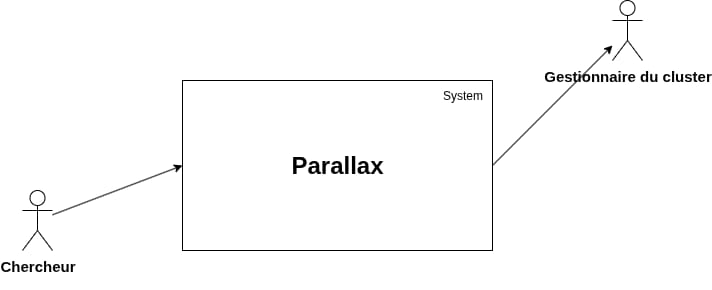
\includegraphics[width=1\textwidth]{images/parallax - diagramme de context.jpeg}
    \caption{Diagramme de Contexte}
    \label{fig:diagramme_contexte}
\end{figure}

\textbf{Exigences fonctionnelles :}
\begin{itemize}
    \item Soumission et exécution distribuée de tâches de calcul (Chercheur).
    \item Import et annotation de programmes via interface CLI (Chercheur).
    \item Consultation des résultats d'exécution avec détails (durée, date) (Chercheur).
    \item Supervision en temps réel de l'état des nœuds via interface Web (Gestionnaire de cluster).
    \item Gestion dynamique du cluster : ajout et retrait de machines (Gestionnaire de cluster).
\end{itemize}

\textbf{Exigences non fonctionnelles :}
\begin{itemize}
    \item Résilience aux pannes : détection automatique et réaffectation des tâches, y compris en cas de surcharge d'un nœud.
    \item Transparence pour le développeur : parallélisation via annotations sans gestion manuelle du réseau.
    \item Légèreté : adaptation aux petits clusters hétérogènes à ressources modestes.
    \item Performance : optimisation de la distribution des tâches en fonction d'un score pondéré des nœuds (CPU, RAM, latence, fréquence), et prise en compte de la latence réseau afin de minimiser les temps de communication entre les machines.
\end{itemize}

\subsection{Diagramme de cas d'utilisation}

Le domaine du calcul distribué académique présente six exigences fondamentales. Le système doit fournir de la puissance de calcul pour les simulations et l'entraînement de modèles d'intelligence artificielle (ED-1). Il doit réduire les coûts d'infrastructure en proposant une alternative aux plateformes cloud distantes (ED-2). Il doit s'affranchir de la dépendance à une connexion Internet souvent instable dans le contexte camerounais (ED-3). Il doit permettre la mutualisation des machines existantes sous-utilisées sur le campus (ED-4). Il doit offrir une soumission de programmes sans expertise réseau, via un mécanisme d'annotations (ED-5). Enfin, il doit assurer la supervision et la maintenance continues du cluster par un administrateur (ED-6).

\begin{figure}[H]
    \centering
    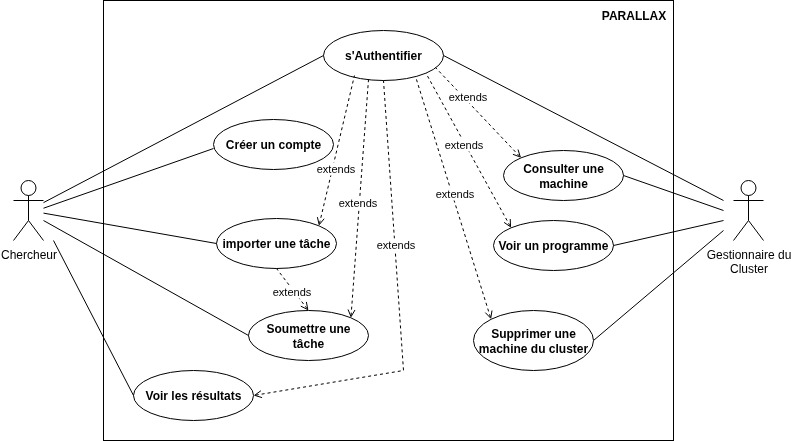
\includegraphics[width=\textwidth,height=\textheight,keepaspectratio]{images/Diagramme UC.jpg.jpeg}
    \caption{Diagramme de cas d'utilisation}
    \label{fig:use_case}
\end{figure}

Le cas d'utilisation « S'authentifier » constitue le point d'entrée commun. Les cas « Créer un compte », « Importer une tâche », « Soumettre une tâche » et « Voir les résultats » concernent le Chercheur. Les cas « Consulter une machine », « Voir un programme » et « Supprimer une machine du cluster » concernent le Gestionnaire du cluster.

\clearpage

\begin{table}[H]
\centering
\renewcommand{\arraystretch}{1.3}
\begin{tabular}{|p{4cm}|p{11cm}|}
\hline
\textbf{Objectif} & Accéder aux fonctionnalités du système \\
\hline
\textbf{Acteur(s)} & Chercheur, Gestionnaire du cluster \\
\hline
\textbf{Pré-condition} & Aucune \\
\hline
\textbf{Scénario nominal} &
\begin{enumerate}
    \item L'acteur entre ses informations d'identification dans le système.
    \item Le système vérifie l'exactitude des informations.
    \item Les informations sont correctes, le système accorde l'accès aux fonctionnalités correspondantes au statut de l'utilisateur.
\end{enumerate} \\
\hline
\textbf{Scénarios alternatifs} &
\begin{itemize}
    \item \textbf{A1 : Erreur de saisie} — Le système informe l'utilisateur et demande de nouvelles informations.
    \item \textbf{A2 : Erreur de connexion à la base de données} — Le système renvoie un message d'erreur.
\end{itemize} \\
\hline
\textbf{Post-condition} & Accès aux fonctionnalités liées au statut de l'utilisateur \\
\hline
\end{tabular}
\caption{Cas d'utilisation : Authentification}
\label{tab:authentification}
\end{table}

\begin{table}[H]
\centering
\renewcommand{\arraystretch}{1.3}
\begin{tabular}{|p{4cm}|p{11cm}|}
\hline
\textbf{Objectif} & Créer un compte utilisateur \\
\hline
\textbf{Acteur(s)} & Chercheur \\
\hline
\textbf{Pré-condition} & Être authentifié \\
\hline
\textbf{Scénario nominal} &
\begin{enumerate}
    \item L'acteur entre ses informations dans le formulaire et le soumet au système.
    \item Le système vérifie l'exactitude des informations.
    \item Le système sauvegarde les informations et renvoie un message de succès.
\end{enumerate} \\
\hline
\textbf{Scénarios alternatifs} &
\begin{itemize}
    \item \textbf{A1 : Erreur de saisie} — Le système demande à l'utilisateur de ressaisir ses informations.
    \item \textbf{A2 : Erreur de connexion à la base de données} — Le système renvoie un message d'erreur.
\end{itemize} \\
\hline
\textbf{Post-condition} & Création du compte utilisateur \\
\hline
\end{tabular}
\caption{Cas d'utilisation : Création de compte}
\label{tab:create_account}
\end{table}

\begin{table}[H]
\centering
\renewcommand{\arraystretch}{1.3}
\begin{tabular}{|p{4cm}|p{11cm}|}
\hline
\textbf{Objectif} & Importer une tâche annotée \\
\hline
\textbf{Acteur(s)} & Chercheur \\
\hline
\textbf{Pré-condition} & Être authentifié \\
\hline
\textbf{Scénario nominal} &
\begin{enumerate}
    \item L'utilisateur clique sur l'option d'importation d'une tâche.
    \item Le système lui permet de sélectionner le dossier ou fichier annoté via un sélecteur de ressources.
    \item L'utilisateur sélectionne et valide.
    \item La tâche est enregistrée dans le système.
\end{enumerate} \\
\hline
\textbf{Scénarios alternatifs} &
\begin{itemize}
    \item \textbf{A1 : Document invalide} — Le système annule l'importation et renvoie un message d'erreur.
\end{itemize} \\
\hline
\textbf{Post-condition} & Dossier / fichier importé dans le système \\
\hline
\end{tabular}
\caption{Cas d'utilisation : Importation d'une tâche}
\label{tab:import_task}
\end{table}

\begin{table}[H]
\centering
\renewcommand{\arraystretch}{1.3}
\begin{tabular}{|p{4cm}|p{11cm}|}
\hline
\textbf{Objectif} & Soumettre une tâche pour son exécution \\
\hline
\textbf{Acteur(s)} & Chercheur \\
\hline
\textbf{Pré-condition} & La tâche a été importée et le chercheur est authentifié \\
\hline
\textbf{Scénario nominal} &
\begin{enumerate}
    \item L'utilisateur sélectionne la tâche à soumettre et valide.
    \item Le Master, grâce aux annotations, découpe et distribue la tâche à exécuter.
    \item Les Workers exécutent la tâche et renvoient les résultats au Master pour recomposition.
    \item Le Master recompose et renvoie le résultat à l'utilisateur.
\end{enumerate} \\
\hline
\textbf{Scénarios alternatifs} &
\begin{itemize}
    \item \textbf{A1 : Erreur de connexion} — Un message d'erreur de connexion est renvoyé à l'utilisateur.
    \item \textbf{A2 : Dossier/fichier mal annoté} — Le système renvoie un message d'erreur d'annotation.
\end{itemize} \\
\hline
\textbf{Post-condition} & Le résultat de l'exécution est renvoyé à l'utilisateur \\
\hline
\end{tabular}
\caption{Cas d'utilisation : Soumission d'une tâche}
\label{tab:submit_task}
\end{table}

\begin{table}[H]
\centering
\renewcommand{\arraystretch}{1.3}
\begin{tabular}{|p{4cm}|p{11cm}|}
\hline
\textbf{Objectif} & Permettre à l'utilisateur de consulter les résultats de ses tâches exécutées \\
\hline
\textbf{Acteur(s)} & Chercheur \\
\hline
\textbf{Pré-condition} & Être authentifié \\
\hline
\textbf{Scénario nominal} &
\begin{enumerate}
    \item L'utilisateur sélectionne le menu des résultats.
    \item Le système affiche les résultats et les détails d'exécution (durée, date, etc.).
\end{enumerate} \\
\hline
\textbf{Scénarios alternatifs} &
\begin{itemize}
    \item \textbf{A1 : Aucun résultat} — Le système affiche un message indiquant l'absence de résultats.
    \item \textbf{A2 : Erreur de récupération} — Un message d'erreur est renvoyé à l'utilisateur.
\end{itemize} \\
\hline
\textbf{Post-condition} & Les résultats sont affichés à l'utilisateur \\
\hline
\end{tabular}
\caption{Cas d'utilisation : Consultation des résultats}
\label{tab:view_results}
\end{table}

\begin{table}[H]
\centering
\renewcommand{\arraystretch}{1.3}
\begin{tabular}{|p{4cm}|p{11cm}|}
\hline
\textbf{Objectif} & Consulter l'état d'une machine du cluster \\
\hline
\textbf{Acteur(s)} & Gestionnaire du cluster \\
\hline
\textbf{Pré-condition} & Être authentifié \\
\hline
\textbf{Scénario nominal} &
\begin{enumerate}
    \item L'utilisateur sélectionne l'option de consultation des machines.
    \item Le système affiche la liste des machines du cluster.
    \item L'utilisateur sélectionne la machine souhaitée.
    \item Le système affiche les détails de la machine sélectionnée.
\end{enumerate} \\
\hline
\textbf{Scénarios alternatifs} &
\begin{itemize}
    \item \textbf{A1 : Machine indisponible} — Le système affiche un message d'erreur d'accessibilité.
    \item \textbf{A2 : Liste vide} — Le système indique qu'aucune machine n'est disponible.
\end{itemize} \\
\hline
\textbf{Post-condition} & Les détails de la machine sont affichés \\
\hline
\end{tabular}
\caption{Cas d'utilisation : Consultation d'une machine}
\label{tab:view_machine}
\end{table}

\begin{table}[H]
\centering
\renewcommand{\arraystretch}{1.3}
\begin{tabular}{|p{4cm}|p{11cm}|}
\hline
\textbf{Objectif} & Déconnecter une machine du cluster \\
\hline
\textbf{Acteur(s)} & Gestionnaire du cluster \\
\hline
\textbf{Pré-condition} & Être authentifié \\
\hline
\textbf{Scénario nominal} &
\begin{enumerate}
    \item L'utilisateur sélectionne la machine à arrêter dans la liste.
    \item L'utilisateur déclenche la commande d'arrêt distant.
    \item Le système demande à l'agent sur la machine d'exécuter la commande d'arrêt.
    \item L'état de la machine est mis à jour sur l'interface pour confirmer l'arrêt.
\end{enumerate} \\
\hline
\textbf{Scénarios alternatifs} &
\begin{itemize}
    \item \textbf{A1 : Échec de communication} — Le système affiche un message d'échec et propose de réessayer.
    \item \textbf{A2 : Refus de confirmation} — L'utilisateur annule, la procédure est abandonnée sans modification.
    \item \textbf{A3 : Machine en cours d'exécution critique} — Le système demande une confirmation supplémentaire ou bloque l'action.
\end{itemize} \\
\hline
\textbf{Post-condition} & La machine est arrêtée (déconnectée du cluster) \\
\hline
\end{tabular}
\caption{Cas d'utilisation : Suppression d'une machine du cluster}
\label{tab:delete_machine}
\end{table}

\begin{table}[H]
\centering
\renewcommand{\arraystretch}{1.3}
\begin{tabular}{|p{4cm}|p{11cm}|}
\hline
\textbf{Objectif} & Voir en temps réel l'état d'un programme en cours d'exécution \\
\hline
\textbf{Acteur(s)} & Gestionnaire du cluster \\
\hline
\textbf{Pré-condition} & Être authentifié \\
\hline
\textbf{Scénario nominal} &
\begin{enumerate}
    \item L'utilisateur sélectionne l'option de consultation des tâches en cours.
    \item Le système affiche la liste des tâches actives.
    \item L'utilisateur sélectionne la tâche souhaitée.
    \item Le système affiche les détails d'exécution (machines impliquées, pourcentage d'avancement, etc.).
\end{enumerate} \\
\hline
\textbf{Scénarios alternatifs} &
\begin{itemize}
    \item \textbf{A1 : Aucune tâche en cours} — Le système affiche un message d'absence de tâches actives.
    \item \textbf{A2 : Erreur de récupération} — Le système affiche un message d'erreur et propose de réessayer.
\end{itemize} \\
\hline
\textbf{Post-condition} & Les détails d'exécution de la tâche sont affichés \\
\hline
\end{tabular}
\caption{Cas d'utilisation : Consultation d'un programme en cours d'exécution}
\label{tab:view_program}
\end{table}

\subsection{Identification des agents}

L'examen des cas d'utilisation révèle trois entités autonomes aux responsabilités distinctes.

\begin{table}[H]
\centering
\renewcommand{\arraystretch}{1.3}
\begin{tabular}{|p{4.5cm}|p{5.5cm}|c|}
\hline
\textbf{Groupement fonctionnel} & \textbf{Justification d'autonomie} & \textbf{Agent} \\
\hline
Gérer la réception, décomposition et recomposition des calculs & Vision globale du calcul et des ressources & \texttt{<<Agent>>} Master \\
\hline
Exécuter des calculs locaux & Autonomie d'exécution, capacité de refus selon charge & \texttt{<<Agent>>} Worker \\
\hline
Superviser l'état du réseau et détecter les pannes & Observation indépendante du flux de calcul & \texttt{<<Agent>>} Contrôleur \\
\hline
\end{tabular}
\caption{Identification des agents}
\label{tab:identification_agents}
\end{table}

L'Agent Master assume les fonctions de point d'entrée utilisateur, de décomposition des calculs, d'orchestration de leur répartition et d'agrégation des résultats. L'Agent Worker est responsable de l'exécution locale des sous-calculs qui lui sont confiés ; chaque machine physique héberge une instance de cet agent. L'Agent Contrôleur maintient une vision globale de l'état du système et détecte les anomalies.

\subsection{Identification des rôles}

\begin{table}[H]
\centering
\renewcommand{\arraystretch}{1.3}
\begin{tabular}{|l|l|l|}
\hline
\textbf{Agent} & \textbf{Rôle} & \textbf{Responsabilité observable} \\
\hline
\multirow{4}{*}{Master} & Réceptionniste & Accueillir et valider les programmes soumis \\
 & Générateur & Transformer un programme annoté en unités distribuables \\
 & Orchestrateur & Décider de l'allocation des sous-tâches aux Workers \\
 & Synthétiseur & Combiner les résultats partiels en résultat final \\
\hline
\multirow{2}{*}{Worker} & Exécuteur & Réaliser le calcul local et signaler la terminaison \\
 & Signaleur d'état & Émettre périodiquement les métriques de charge \\
\hline
\multirow{2}{*}{Contrôleur} & Observateur & Collecter et centraliser les informations d'état \\
 & Détecteur de panne & Identifier les anomalies et alerter les agents concernés \\
\hline
\end{tabular}
\caption{Identification des rôles}
\label{tab:identification_roles}
\end{table}

\subsection{Identification du SMA}

\subsubsection{Organisation}

L'organisation est hiérarchique fonctionnelle sans contrôle autoritaire. Le Master coordine mais ne commande pas : il propose des sous-calculs aux Workers qui conservent le droit de refuser. Le Contrôleur observe sans intervenir dans le flux de calcul. Cette organisation émerge des dépendances naturelles : le Master dépend des Workers pour l'exécution, les Workers dépendent du Master pour l'obtention des tâches, et le Master dépend du Contrôleur pour une vision fiable des ressources.

Tous les agents partagent le même objectif global — l'exécution efficace des calculs — mais avec des points de vue partiels. Le Master a une vue globale du calcul mais pas de l'état réseau en temps réel. Le Worker a une vue locale de sa charge mais ignore la charge des autres. Le Contrôleur a une vue globale de la présence des nœuds mais ignore la sémantique des calculs.

\subsubsection{Environnement}

L'environnement est un réseau local académique aux caractéristiques contraignantes. La couche physique comprend un switch Ethernet à cinq ports et six câbles RJ45 sertis manuellement, limitant l'extension à six nœuds. La latence est faible mais la bande passante est modeste. L'absence de redondance réseau fait du switch un point de défaillance unique.

La couche informatique est hétérogène : trois machines DELL sous Ubuntu Server 18.04 avec des processeurs Intel Core 2 Duo et des mémoires de 2 à 4 Go ; trois thin clients Wyse sous Windows CE avec 32 à 64 Mo de RAM et des processeurs de 533 MHz à 1 GHz.

Chaque agent perçoit son environnement via les métriques locales de sa machine ($LOAD_v$, $NET_v$) et via les messages reçus des autres agents. Il agit sur l'environnement en envoyant des messages TCP, en exécutant des calculs localement ou en modifiant l'état du cluster via les mécanismes d'élection et d'enregistrement.

L'environnement est dynamique : ajout et retrait volontaires par le Gestionnaire, pannes et surcharges imprévues, connectivité Internet externe instable rendant le cluster autonome une nécessité.

\subsubsection{Interaction}

Les interactions se déclinent en trois types.

La \textbf{communication} est l'échange structuré d'informations : heartbeat du Worker vers le Contrôleur toutes les deux secondes, messages de sous-calcul du Master vers le Worker, résultats partiels en retour, gossip inter-pairs pour la diffusion progressive de l'état du cluster. Un Worker refuse une tâche lorsque $LOAD_v.cpuusage \geq \theta_{high}$ ou que sa file de tâches est saturée ; dans ce cas il renvoie un message de refus et le Master sélectionne un autre nœud disponible.

La \textbf{coordination} gère les dépendances temporelles et les accès aux ressources : barrière de synchronisation attendant tous les résultats avant recomposition, élection du nœud remplaçant lors d'une défaillance, score pondéré pour l'allocation et la hiérarchisation des nœuds.

La \textbf{coopération} est le travail collectif vers l'objectif partagé : division du travail par décomposition des programmes annotés, partage d'information via le Contrôleur pour les décisions d'allocation, assistance mutuelle par migration des tâches lors d'une panne de Worker.

\subsubsection{Séquences système}

\begin{figure}[H]
    \centering
    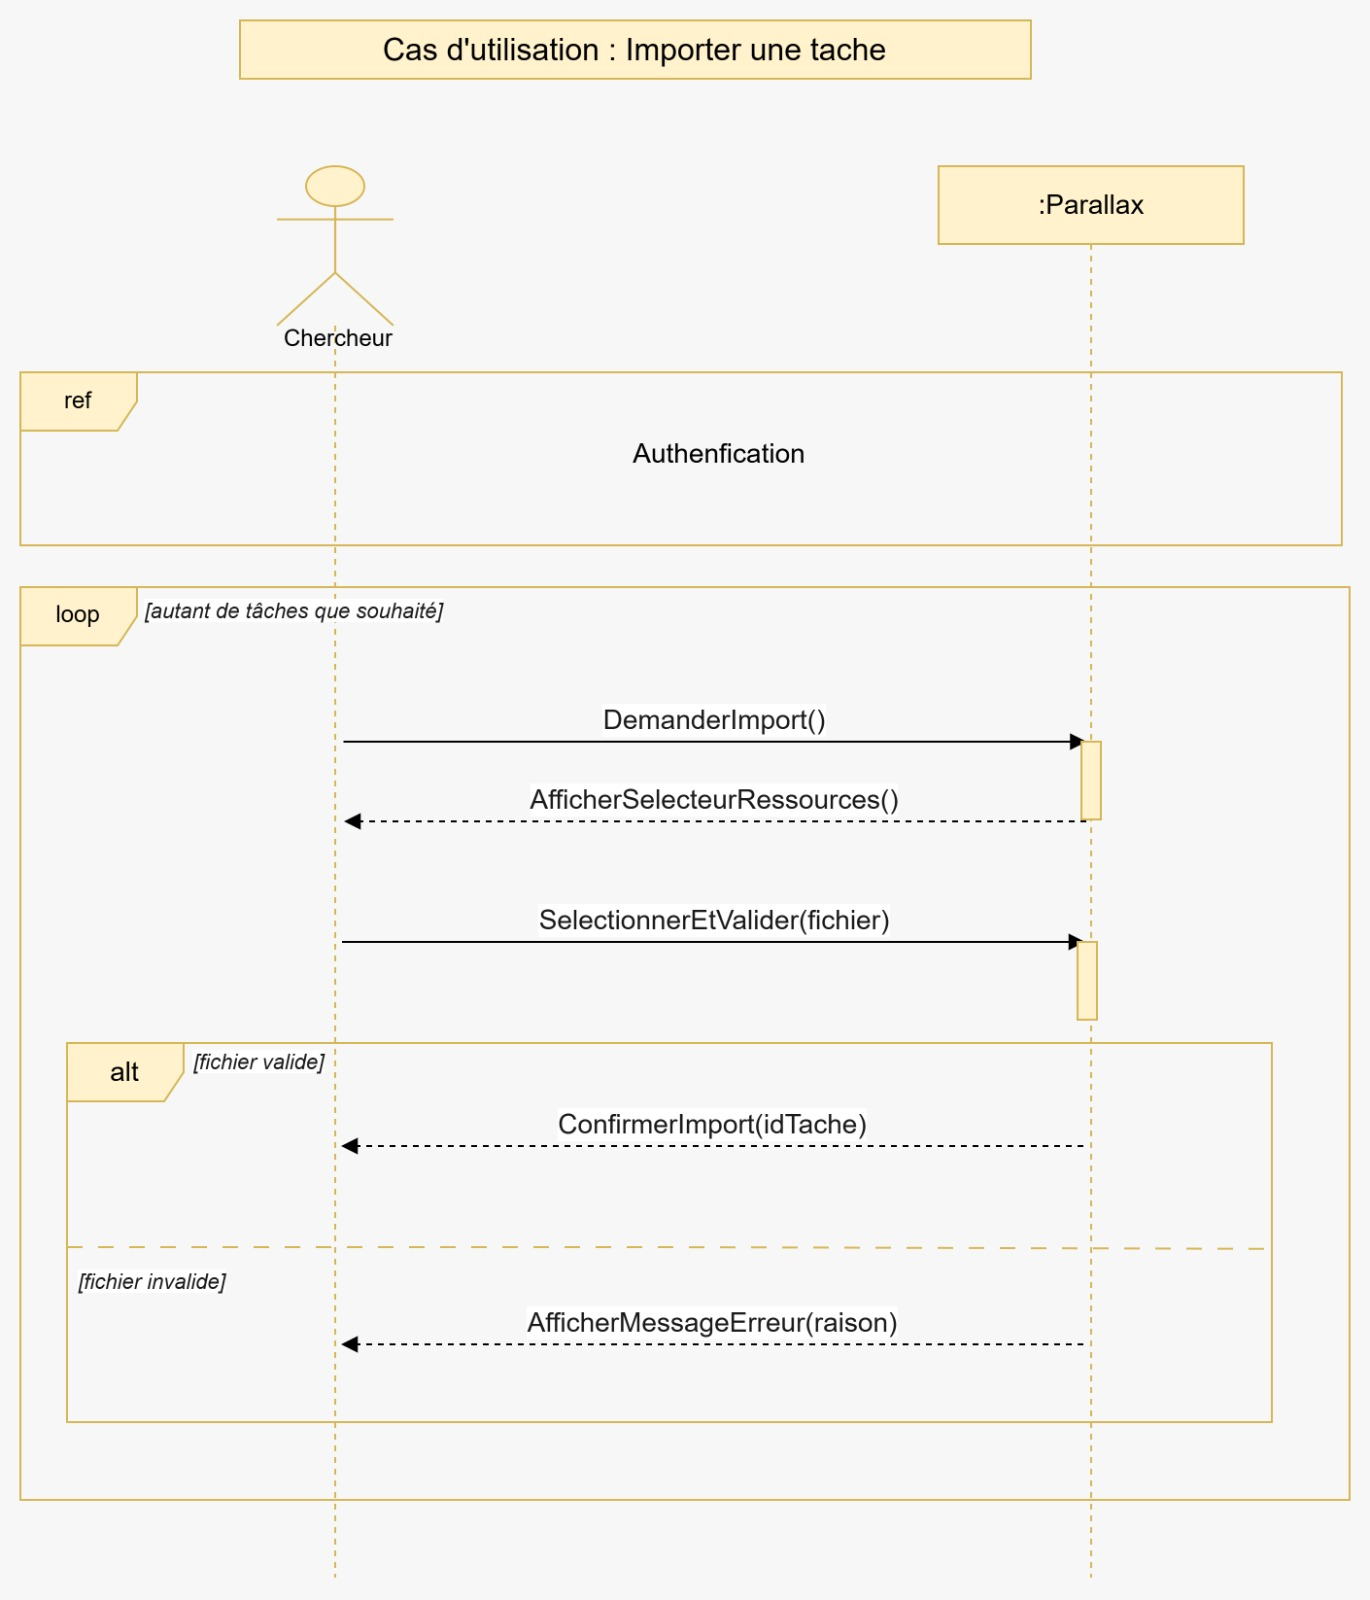
\includegraphics[width=1\textwidth]{images/diagramme de sequences - importer une tache - parallax .jpeg}
    \caption{Diagramme de séquences système — Importer une tâche}
    \label{fig:seq_import}
\end{figure}

\begin{figure}[H]
    \centering
    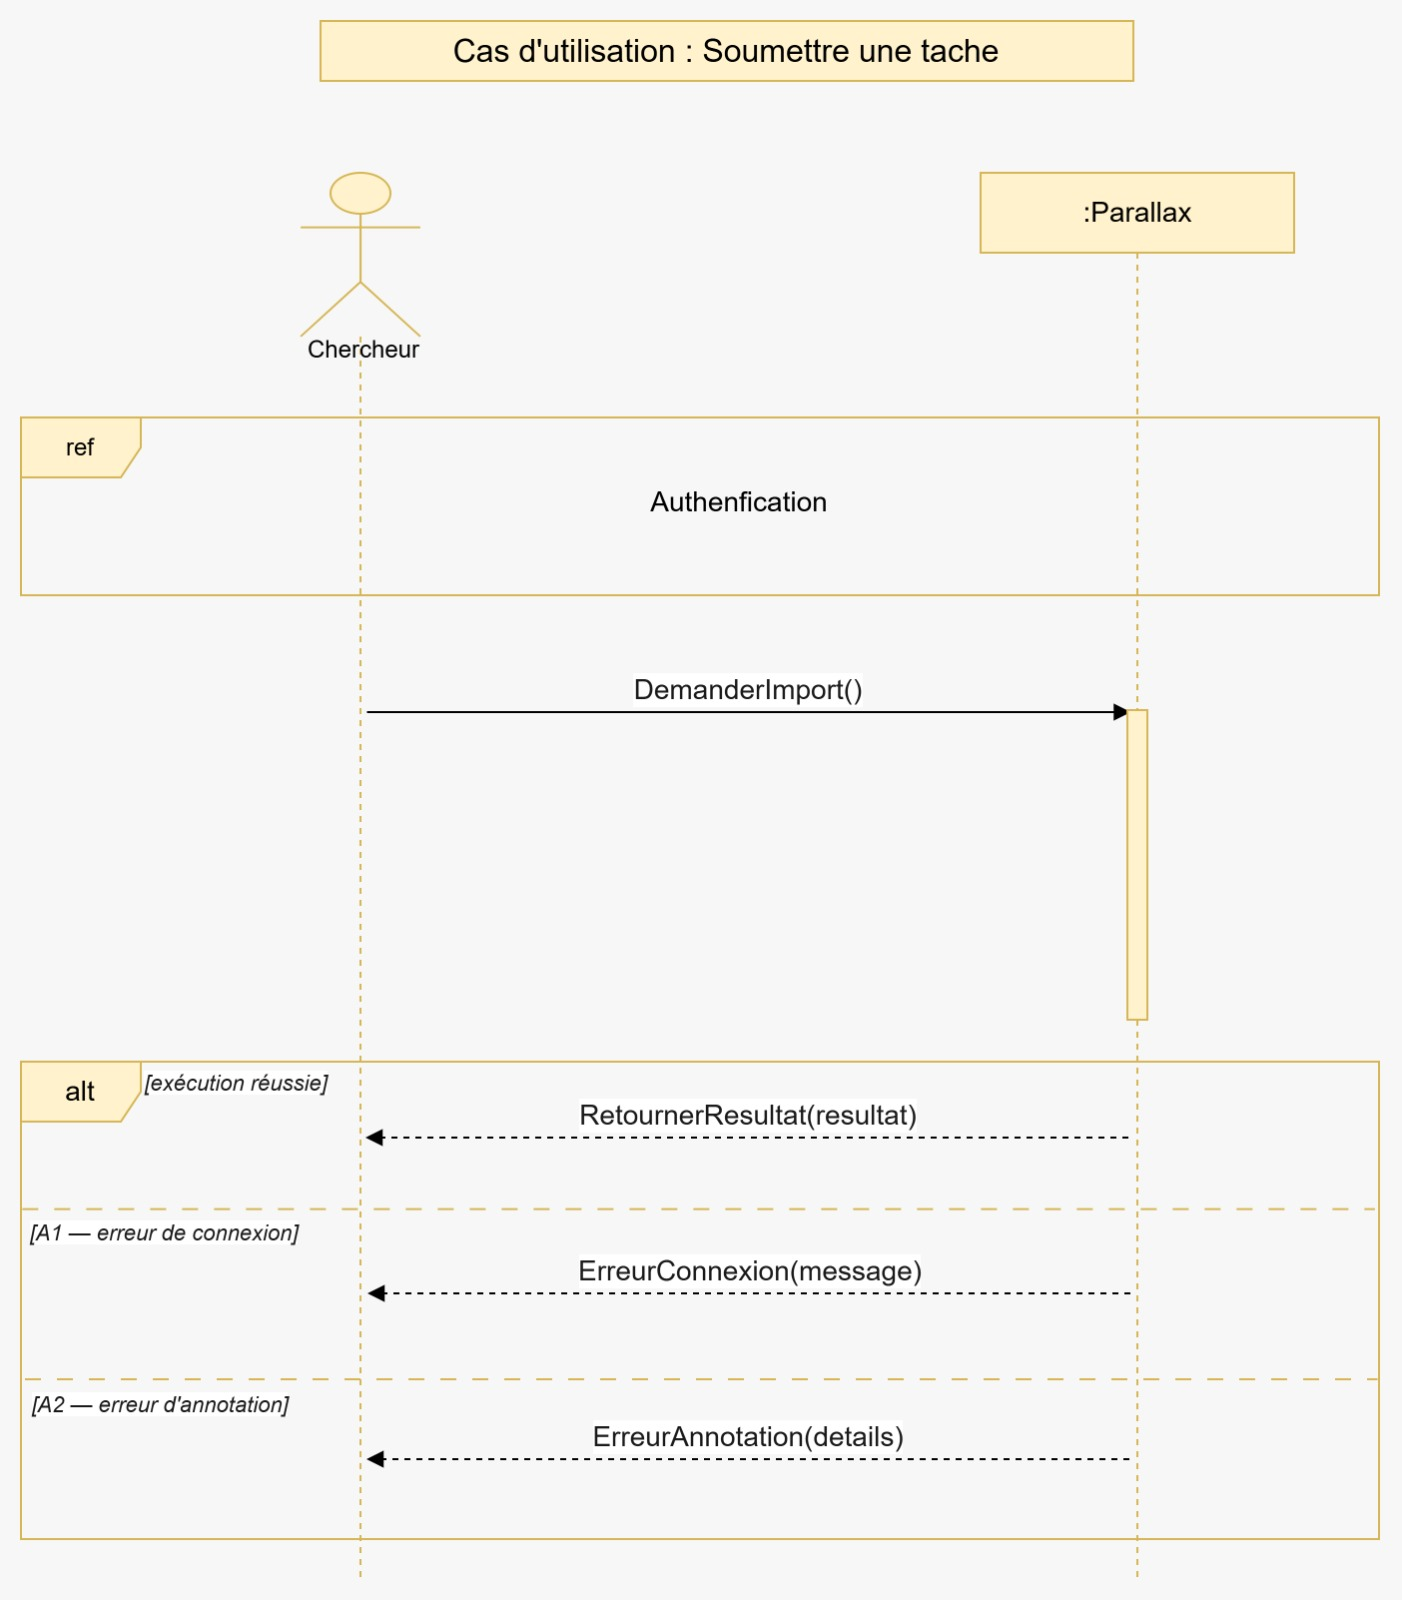
\includegraphics[width=1\textwidth]{images/diagramme de sequence - soumettre une tache- parallax.jpeg}
    \caption{Diagramme de séquences système — Soumettre une tâche}
    \label{fig:seq_soumettre}
\end{figure}

\begin{figure}[H]
    \centering
    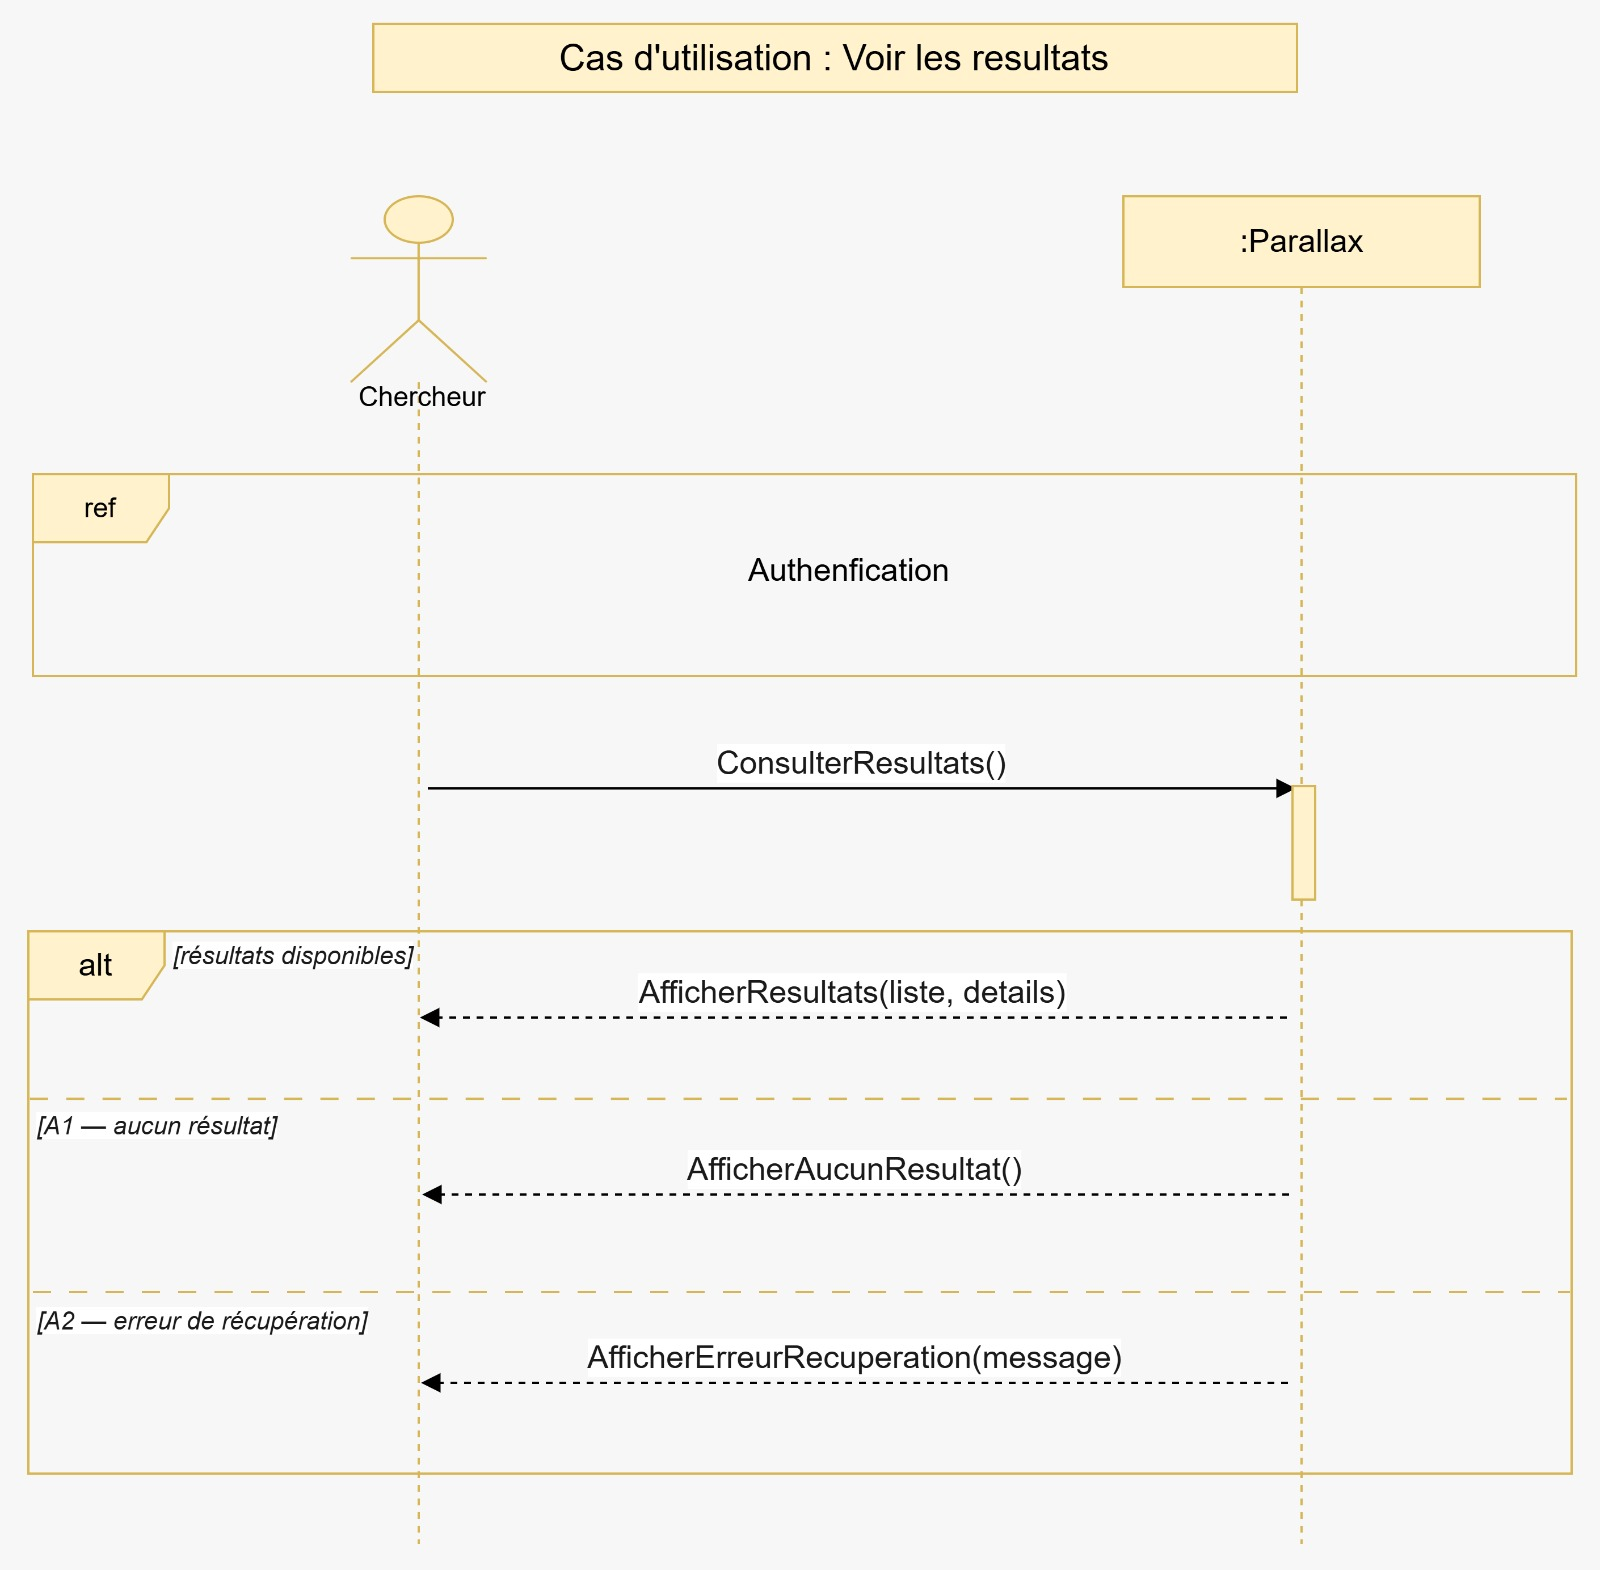
\includegraphics[width=1\textwidth]{images/sequence systeme - voir les resultats.jpeg}
    \caption{Diagramme de séquences système — Voir les résultats}
    \label{fig:seq_resultats}
\end{figure}

\begin{figure}[H]
    \centering
    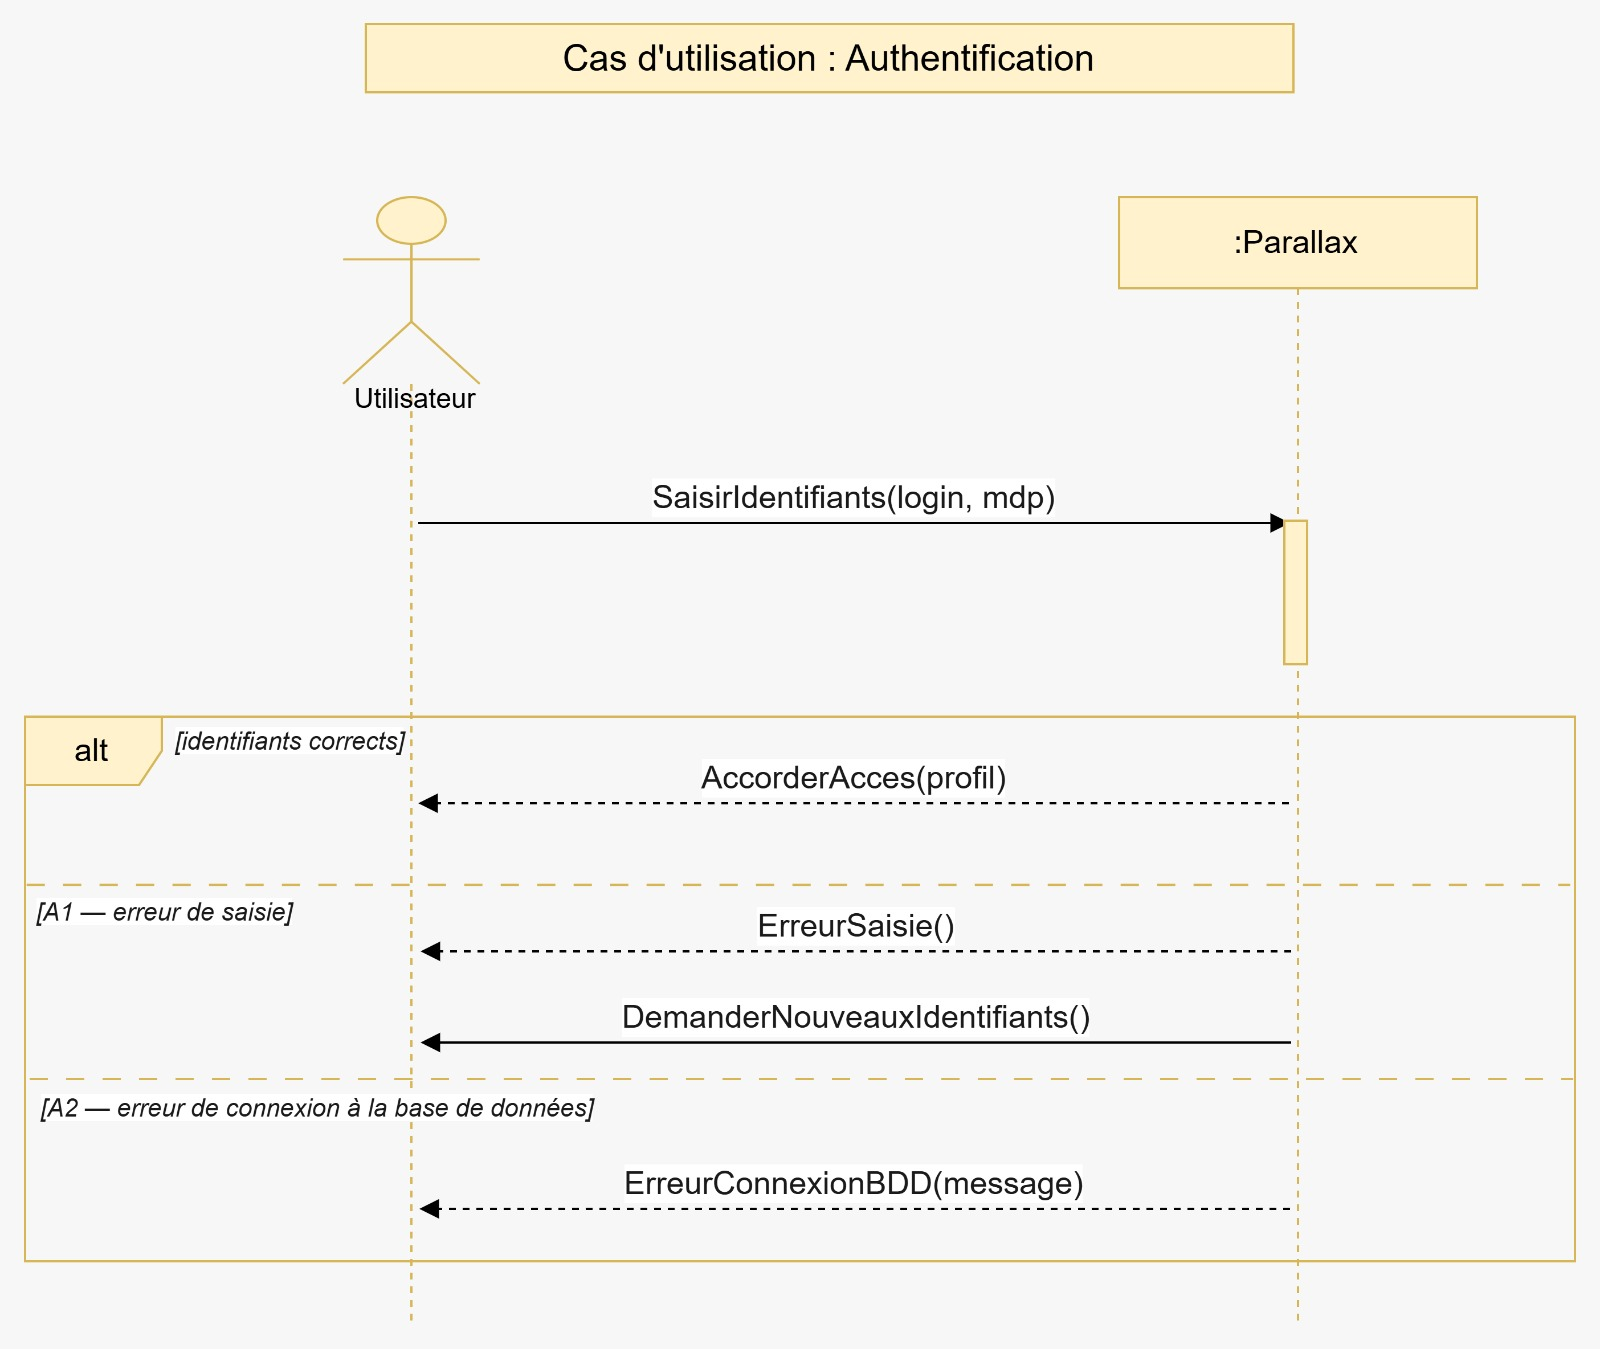
\includegraphics[width=1\textwidth]{images/diagramme de sequences systeme - authhentification - parallax.jpeg}
    \caption{Diagramme de séquences système — Authentification}
    \label{fig:seq_auth}
\end{figure}

\begin{figure}[H]
    \centering
    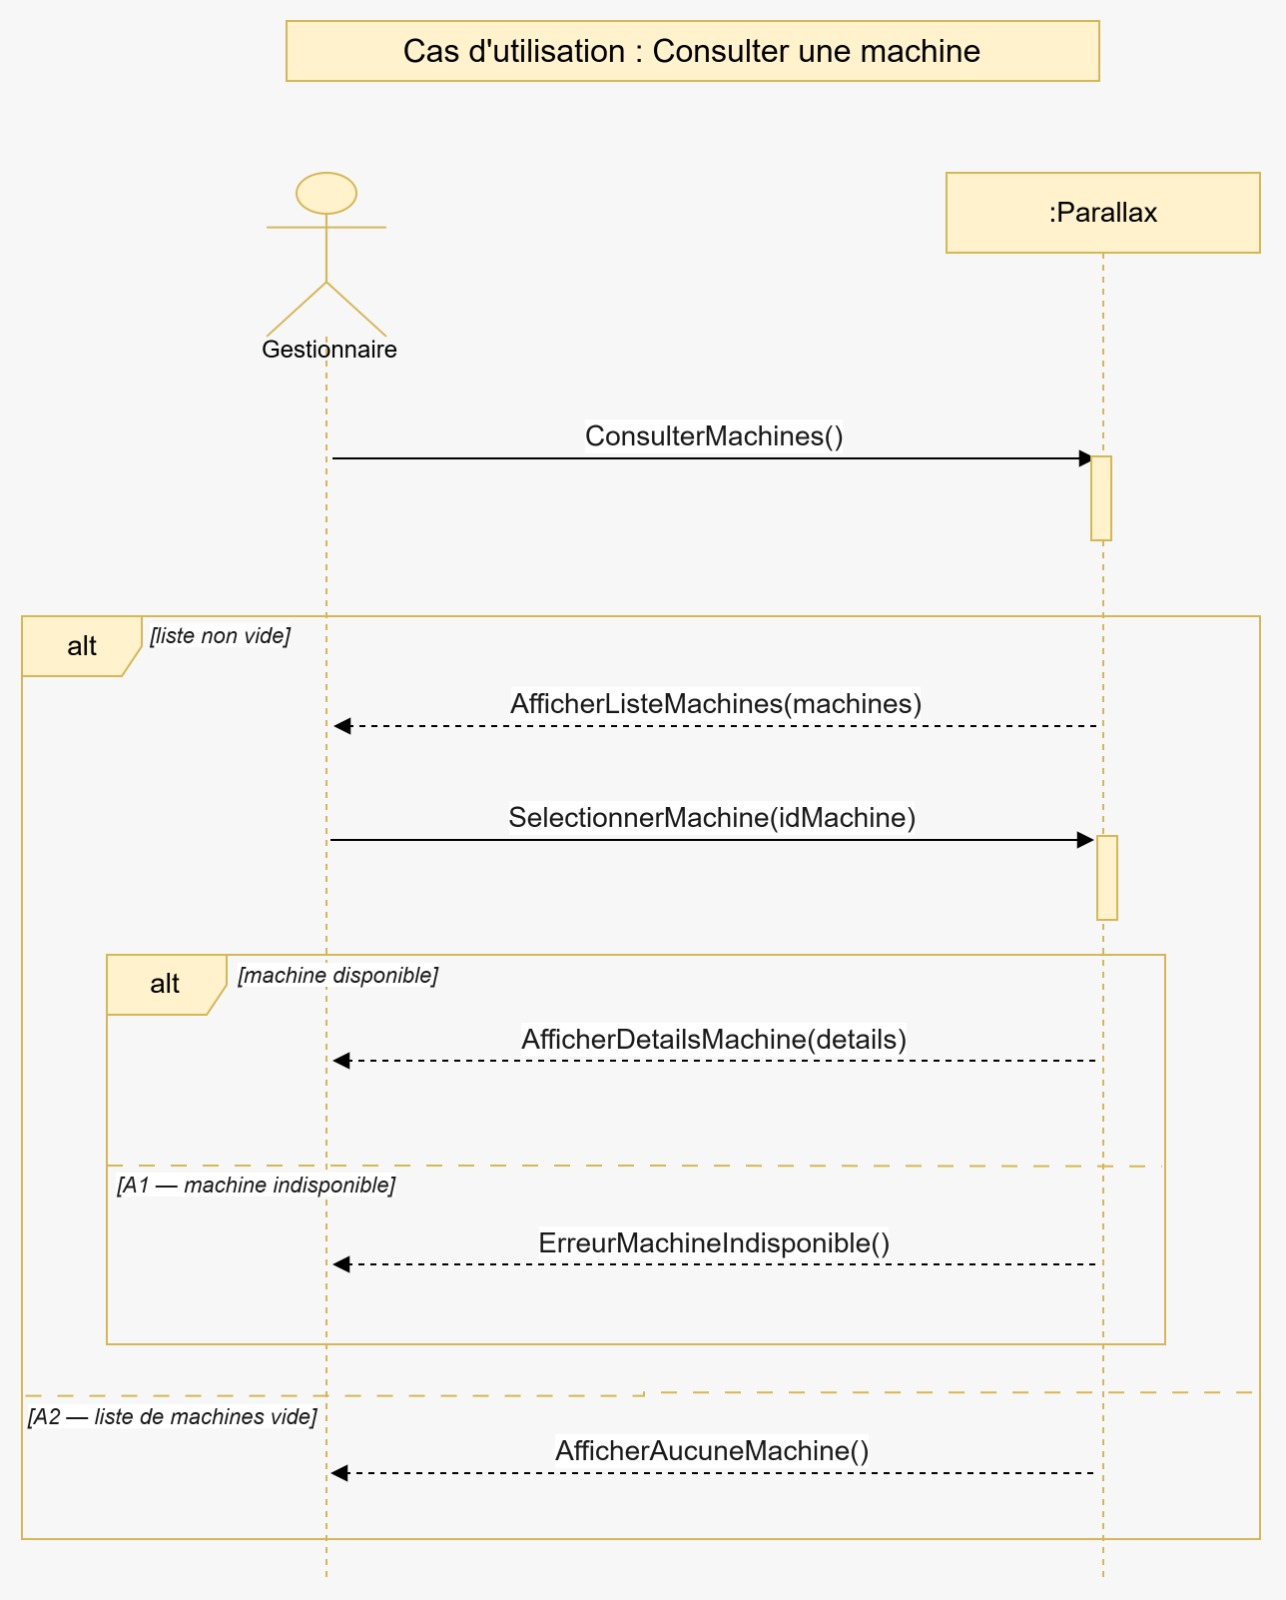
\includegraphics[width=1\textwidth]{images/sequence systeme - consulter une machine.jpeg}
    \caption{Diagramme de séquences système — Consulter une machine}
    \label{fig:seq_machine}
\end{figure}

% ==============================================================================
\section{Conception}
% ==============================================================================

La conception du système SMA\_PARALLAX traduit les éléments identifiés en phase d'analyse en une architecture opérationnelle. Elle définit la structure des agents, leurs comportements, les protocoles de communication et les mécanismes de coordination distribuée assurant l'exécution des calculs dans un cluster hétérogène.

\subsection{Architecture du SMA}

L'architecture de SMA\_PARALLAX est hiérarchique fonctionnelle à trois niveaux :

\begin{itemize}
    \item \textbf{Niveau supervision} (Contrôleur) : maintient une vue globale cohérente, détecte les pannes, gère l'élection.
    \item \textbf{Niveau coordination} (Master) : reçoit les calculs, décompose, distribue et agrège les résultats.
    \item \textbf{Niveau exécution} (Workers) : réalise les sous-calculs de manière autonome et signale leur état.
\end{itemize}

Cette architecture hybride combine la réactivité du niveau inférieur (heartbeat, détection rapide) et la délibération du niveau supérieur (planification de la distribution, élection du remplaçant).

\begin{figure}[H]
    \centering
    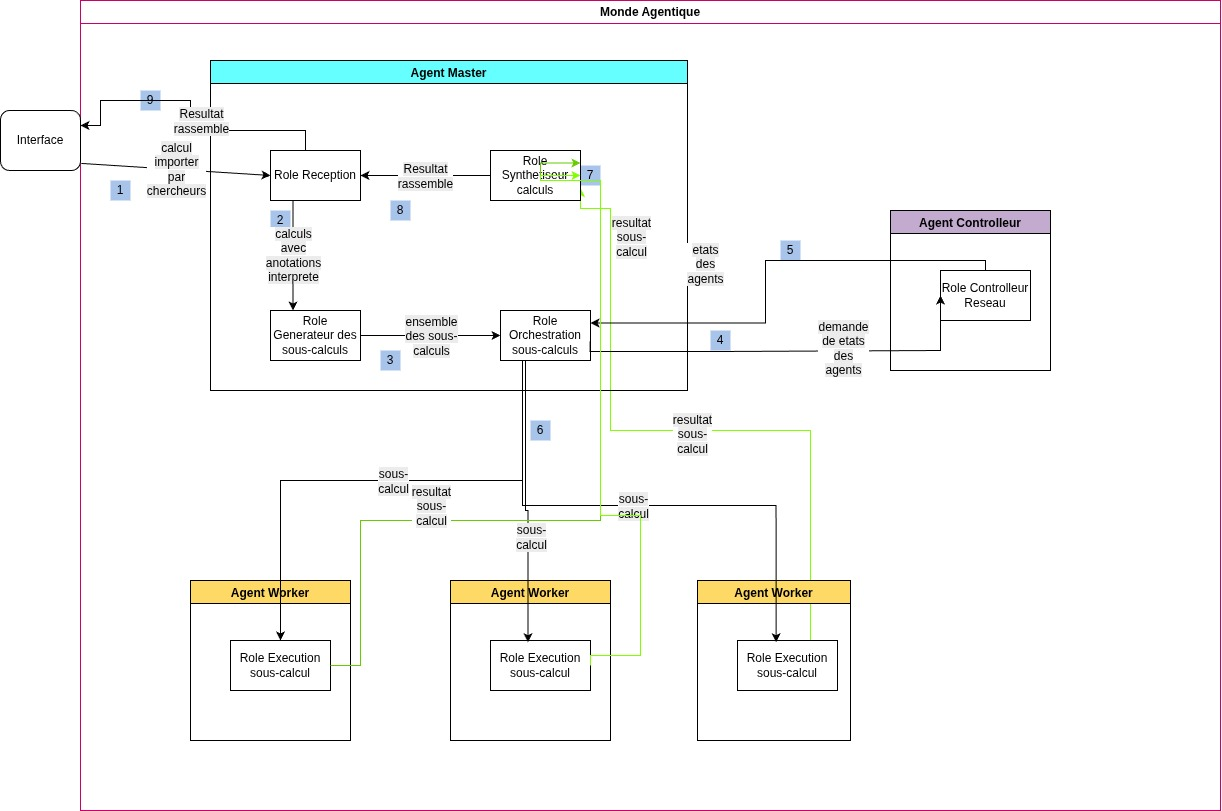
\includegraphics[width=1.0\linewidth]{Architecture_agentique (2).jpg}
    \caption{Architecture agentique de SMA\_PARALLAX}
    \label{fig:architecture_agentique}
\end{figure}

\subsection{Structure de l'agent et du SMA}

\subsubsection{Modélisation physique d'un nœud}

Chaque machine $v \in V_M$ est caractérisée par un vecteur d'état :

\[
X_v =
\begin{bmatrix}
ID_v \\ NET_v \\ COMPUTE_v \\ MEMORY_v \\ STORAGE_v \\
LOAD_v \\ RELIABILITY_v \\ STATE_v \\ SECURITY_v
\end{bmatrix}
\]

\begin{itemize}
    \item[*] $ID_v = (\text{uuid}, \text{role}, \text{region})$ : identité unique, rôle et localisation.
    \item[*] $NET_v = (\text{ip}, \text{latency}, \text{bandwidth}_{in}, \text{bandwidth}_{out}, \text{jitter}, \text{loss})$ : performances réseau.
    \item[*] $COMPUTE_v = (\text{cpucores}, \text{cpufreq}, \text{gpu}, \text{flops})$ : capacités de calcul.
    \item[*] $MEMORY_v = (\text{ram}, \text{mem\_bandwidth})$ : ressources mémoire.
    \item[*] $STORAGE_v = (\text{disk}, \text{io})$ : capacités de stockage.
    \item[*] $LOAD_v = (\text{cpuusage}, \text{ramusage}, \text{queue})$ : charge courante.
    \item[*] $STATE_v = (\text{status}, \text{availability})$ : état opérationnel.
    \item[*] $RELIABILITY_v = (\text{uptime}, \text{failurerate})$ : fiabilité.
    \item[*] $SECURITY_v = (\text{auth}, \text{trust})$ : sécurité et confiance.
\end{itemize}

\subsubsection{Modélisation mentale : architecture BDI des agents cognitifs}

Les agents Master et Contrôleur suivent une architecture BDI (Belief-Desire-Intention) qui structure leur état mental en trois composantes \cite{wooldridge} :

\begin{itemize}
    \item \textbf{Croyances ($B$)} : représentation informationnelle de l'état du monde. Le Master maintient des croyances sur l'état des Workers (charge, disponibilité) via le Contrôleur. Le Contrôleur maintient des croyances sur la présence et la santé de tous les nœuds via les heartbeats.
    \item \textbf{Désirs ($D$)} : états que l'agent souhaite atteindre. Le Master désire minimiser le temps global d'exécution des calculs. Le Contrôleur désire maximiser la disponibilité du cluster.
    \item \textbf{Intentions ($I$)} : engagements délibérés que l'agent poursuit activement. Le Master forme l'intention de distribuer les sous-calculs selon le score pondéré. Le Contrôleur forme l'intention de déclencher une élection lors d'une défaillance critique.
\end{itemize}

Par exemple, lorsque le Contrôleur envoie une alerte de panne d'un Worker en cours d'exécution, le Master révise ses croyances (ce Worker n'est plus disponible), met à jour ses intentions (réaffecter les tâches en cours de ce Worker) et planifie immédiatement leur redistribution vers les nœuds disponibles restants.

L'AgentWorker, de type réactif avec état, ne suit pas le cycle BDI complet : il maintient un état interne minimal ($LOAD_v$) et réagit par règles condition-action sans délibération symbolique.

\subsubsection{Typologie des agents de SMA\_PARALLAX}

\begin{table}[H]
\centering
\renewcommand{\arraystretch}{1.3}
\begin{tabular}{|l|l|p{6cm}|l|}
\hline
\textbf{Agent} & \textbf{Type} & \textbf{Justification} & \textbf{État interne} \\
\hline
AgentWorker & Réactif avec état & Perçoit l'environnement via heartbeat, maintient un état interne (charge, file de tâches), réagit par règles condition-action & $LOAD_v$, file des tâches en cours \\
\hline
AgentMaster & Cognitif orienté but & Représente symboliquement l'état du cluster, planifie la décomposition et la distribution selon un but de minimisation du temps global & Croyances sur le cluster, buts de répartition, intentions de distribution \\
\hline
AgentContrôleur & Cognitif orienté utilité & Évalue les configurations du cluster via une fonction d'utilité (fiabilité, cohérence de la vue globale) & Modèle social des nœuds, historique des pannes \\
\hline
\end{tabular}
\caption{Typologie des agents de SMA\_PARALLAX}
\label{tab:typologie_agents}
\end{table}

\subsubsection{Diagramme de classes}

\begin{figure}[H]
    \centering
    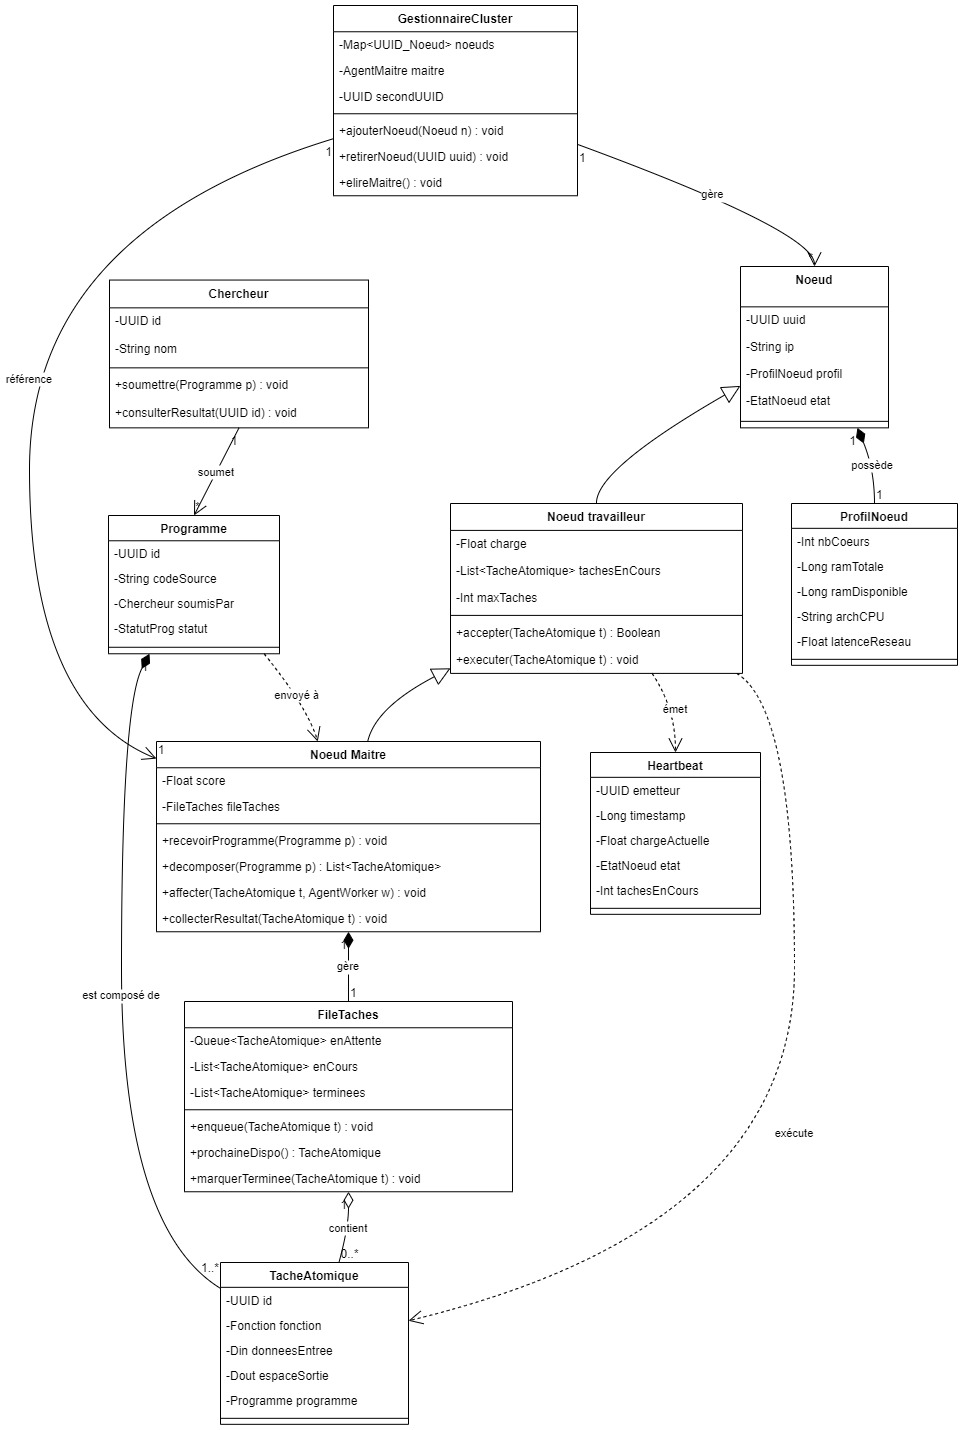
\includegraphics[width=1\textwidth]{images/parralax-classe technique.jpg}
    \caption{Diagramme de classes}
    \label{fig:classes}
\end{figure}

\subsubsection{Actions et événements du système}

\begin{table}[H]
\centering
\renewcommand{\arraystretch}{1.3}
\begin{tabular}{|c|p{3cm}|p{3.5cm}|p{3cm}|p{2cm}|p{2cm}|}
\hline
\textbf{N°} & \textbf{Action} & \textbf{Commentaire} & \textbf{Rôle} & \textbf{Entrée} & \textbf{Sortie} \\
\hline
1 & Réception des calculs & Prise en charge des requêtes & Réception (Master) & Requête utilisateur & Tâche globale \\
\hline
2 & Décomposition & Division en sous-calculs & Génération (Master) & Tâche globale & Sous-calculs \\
\hline
3 & Distribution & Allocation aux Workers & Orchestration (Master) & Sous-calculs + états & Tâches assignées \\
\hline
4 & Réception sous-calcul & Réception par le Worker & Exécution (Worker) & Sous-calcul & Tâche locale \\
\hline
5 & Exécution & Calcul effectif & Exécution (Worker) & Tâche locale & Résultat partiel \\
\hline
6 & Retour résultat & Envoi au Master & Exécution (Worker) & Résultat partiel & Résultat transmis \\
\hline
7 & Agrégation & Combinaison des résultats & Synthèse (Master) & Résultats partiels & Résultat final \\
\hline
8 & Observation & Surveillance ressources & Contrôle (Master) & États agents & Vue système \\
\hline
9 & Diffusion état Worker & Communication charge/dispo & Contrôle (Worker) & État local & Infos d'état \\
\hline
10 & Collecte états & Centralisation des infos & Contrôle (Contrôleur) & Infos d'état & BDD état \\
\hline
11 & Détection pannes & Identification anomalies & Contrôle (Contrôleur) & États système & Alertes \\
\hline
12 & Notification défaillance & Alerte au Master & Contrôle (Contrôleur) & Alertes & Notification \\
\hline
13 & Enregistrement nœud & Ajout au cluster & Contrôle (Contrôleur) & Infos nœud & Nœud enregistré \\
\hline
\end{tabular}
\caption{Table des actions de SMA\_PARALLAX}
\label{tab:actions}
\end{table}

\begin{table}[H]
\centering
\renewcommand{\arraystretch}{1.3}
\begin{tabular}{|c|p{4cm}|p{9cm}|}
\hline
\textbf{N°} & \textbf{Événement} & \textbf{Description} \\
\hline
E1 & Soumission de calcul & Un utilisateur soumet une requête via l'interface. Déclenche l'agent de réception. \\
\hline
E2 & Réception tâche globale & Le Master reçoit et valide la tâche. \\
\hline
E3 & Décomposition déclenchée & La tâche est transformée en sous-calculs. \\
\hline
E4 & Disponibilité des ressources & Les états des Workers orientent la planification. \\
\hline
E5 & Allocation des sous-calculs & Les sous-tâches sont assignées selon le score pondéré. \\
\hline
E6 & Réception sous-calcul & Un Worker reçoit une tâche à exécuter. \\
\hline
E7 & Début d'exécution & Le Worker commence le traitement. \\
\hline
E8 & Fin d'exécution & Le Worker produit un résultat partiel. \\
\hline
E9 & Envoi résultat partiel & Le résultat est transmis au Master. \\
\hline
E10 & Réception résultats partiels & Le Master collecte les résultats des Workers. \\
\hline
E11 & Agrégation & Les résultats partiels sont combinés. \\
\hline
E12 & Production résultat final & Le résultat est prêt à être renvoyé à l'utilisateur. \\
\hline
E13 & Diffusion état Worker & Les Workers envoient périodiquement leur état. \\
\hline
E14 & Collecte des états & Le Contrôleur centralise les informations. \\
\hline
E15 & Détection de défaillance & Une anomalie est détectée. \\
\hline
E16 & Notification de défaillance & Une alerte est envoyée au Master. \\
\hline
E17 & Enregistrement nouveau nœud & Un nouvel agent rejoint le système. \\
\hline
\end{tabular}
\caption{Table des événements de SMA\_PARALLAX}
\label{tab:events}
\end{table}

\subsection{Comportement des agents}

Le comportement des agents est régi par leurs états internes et les transitions déclenchées par les événements du système.

\begin{figure}[H]
    \centering
    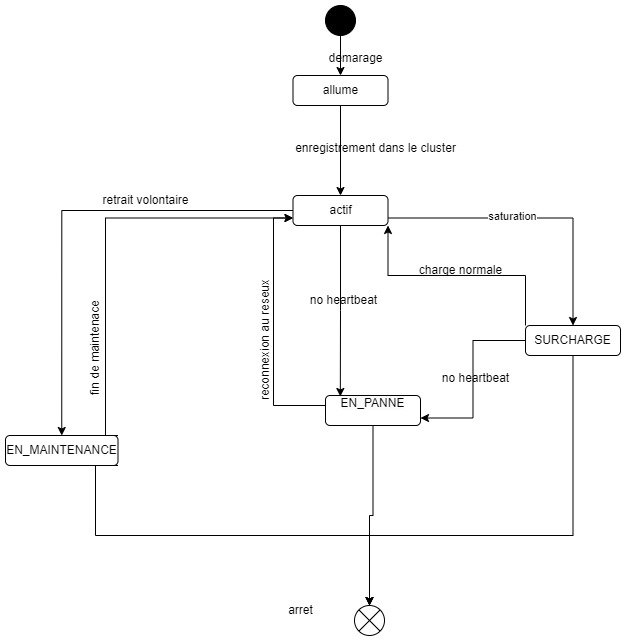
\includegraphics[width=1\textwidth]{images/parralax-etat d'un noeud.jpg}
    \caption{Diagramme d'état d'un nœud}
    \label{fig:etat_noeud}
\end{figure}

\begin{figure}[H]
    \centering
    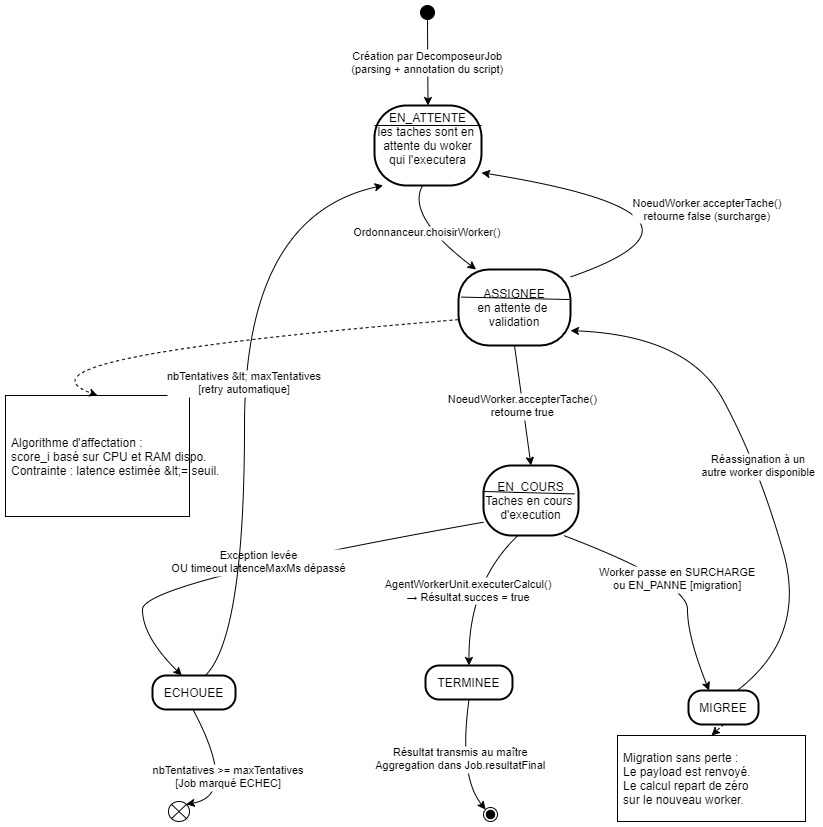
\includegraphics[width=1\textwidth]{images/parralax-etat d'une tache.jpg}
    \caption{Diagramme d'état d'une tâche}
    \label{fig:etat_tache}
\end{figure}

\begin{figure}[H]
    \centering
    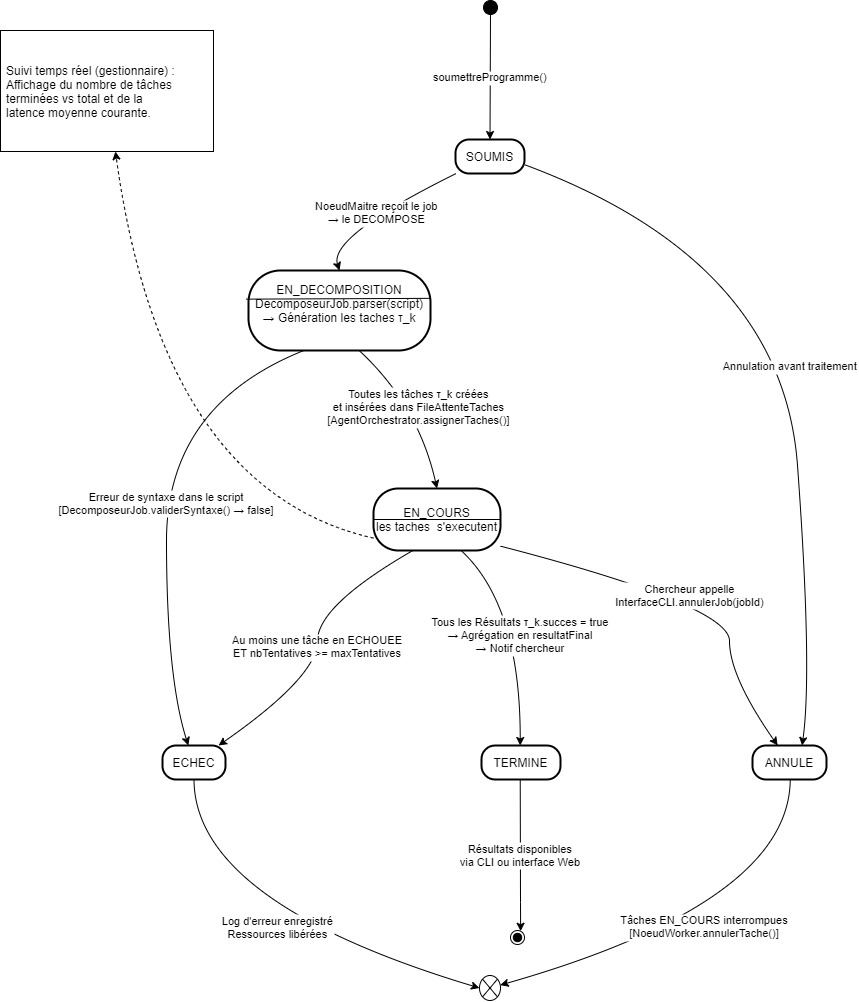
\includegraphics[width=1\textwidth]{images/parralax-etat d'un programme.jpg}
    \caption{Diagramme d'état d'un programme}
    \label{fig:etat_programme}
\end{figure}

\subsection{Description des rôles}

Les diagrammes suivants illustrent les interactions conçues entre les rôles identifiés en analyse.

\begin{figure}[H]
    \centering
    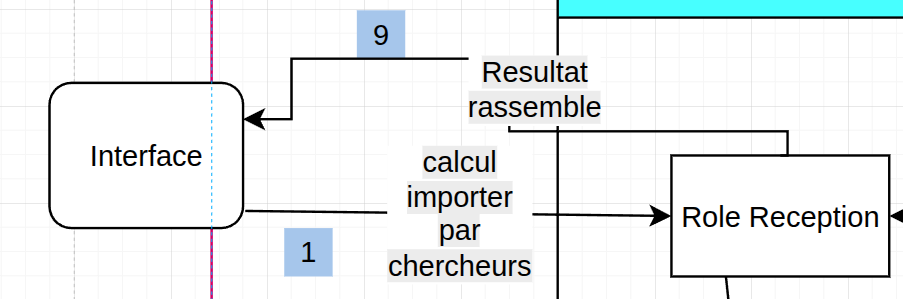
\includegraphics[width=0.5\linewidth]{image.png}
    \caption{Interaction entre le rôle de réception et son environnement}
    \label{fig:interaction_reception_env}
\end{figure}

\begin{figure}[H]
    \centering
    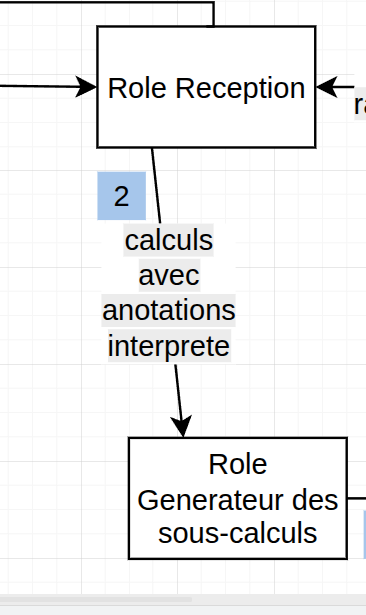
\includegraphics[width=0.5\linewidth]{image2.png}
    \caption{Interaction entre le réceptionniste et le générateur de sous-tâches}
    \label{fig:interaction_reception_generation}
\end{figure}

\begin{figure}[H]
    \centering
    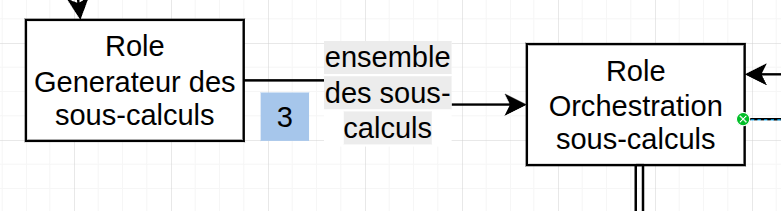
\includegraphics[width=0.5\linewidth]{image3.png}
    \caption{Interaction détaillée entre réception et génération des sous-calculs}
    \label{fig:interaction_detail_generation}
\end{figure}

\begin{figure}[H]
    \centering
    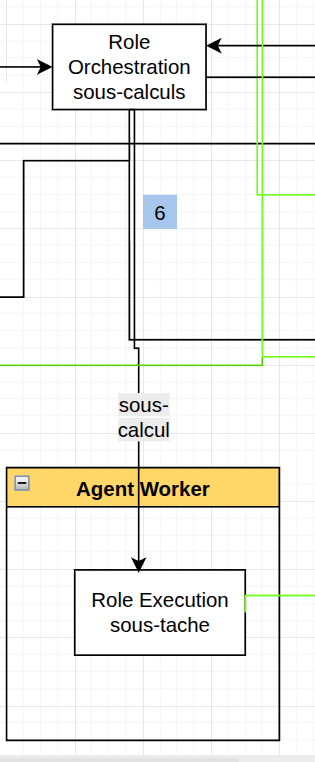
\includegraphics[width=0.5\linewidth]{image4.png}
    \caption{Interaction entre le générateur de sous-calculs et l'orchestrateur}
    \label{fig:interaction_generation_orchestration}
\end{figure}

\begin{figure}[H]
    \centering
    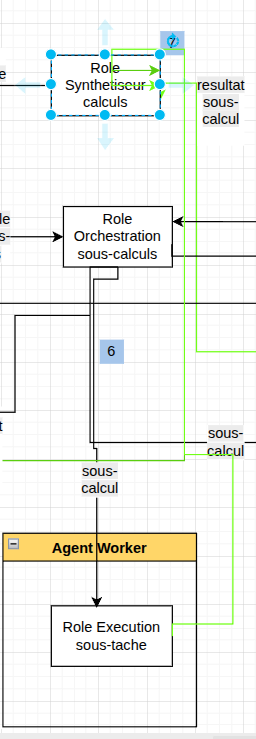
\includegraphics[width=0.5\linewidth]{image5.png}
    \caption{Interaction entre les agents d'exécution et le synthétiseur}
    \label{fig:interaction_execution_synthese}
\end{figure}

\begin{figure}[H]
    \centering
    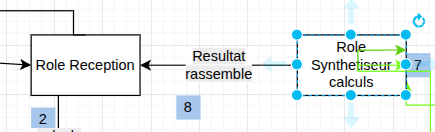
\includegraphics[width=0.5\linewidth]{image6.png}
    \caption{Interaction entre le synthétiseur et le réceptionniste}
    \label{fig:interaction_synthese_reception}
\end{figure}

Les diagrammes de séquences techniques suivants décrivent le comportement détaillé de chaque rôle au niveau de l'implémentation.

\begin{figure}[H]
    \centering
    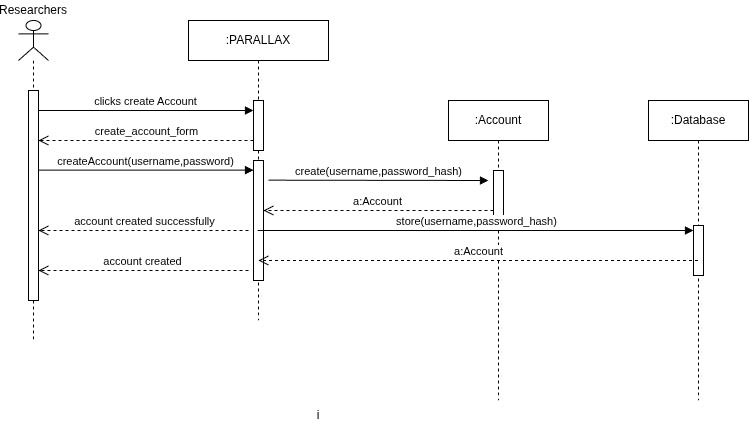
\includegraphics[width=1\textwidth]{images/parallax-AUTHENTIFCATION.jpg.jpeg}
    \caption{Diagramme de séquences technique — Authentification}
    \label{fig:seq_tech_auth}
\end{figure}

\begin{figure}[H]
    \centering
    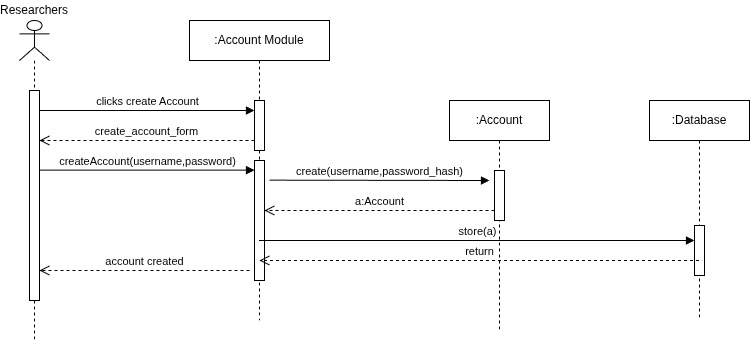
\includegraphics[width=1\textwidth]{images/parallax-CREATE_ACCOUNT.jpg.jpeg}
    \caption{Diagramme de séquences technique — Création de compte}
    \label{fig:seq_tech_account}
\end{figure}

\begin{figure}[H]
    \centering
    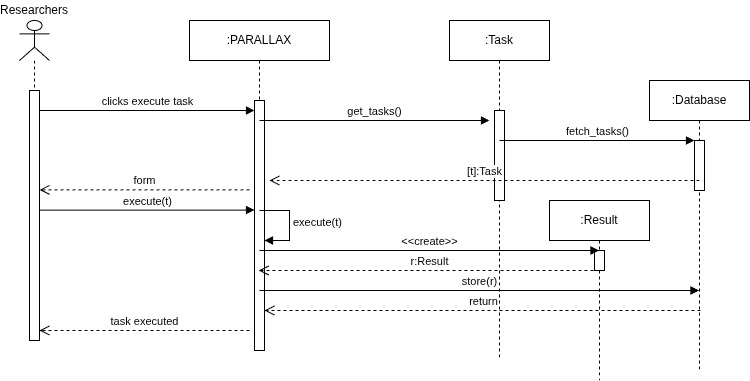
\includegraphics[width=1\textwidth]{images/parallax-ImportTask (2).jpg.jpeg}
    \caption{Diagramme de séquences technique — Importation d'une tâche}
    \label{fig:seq_tech_import}
\end{figure}

\begin{figure}[H]
    \centering
    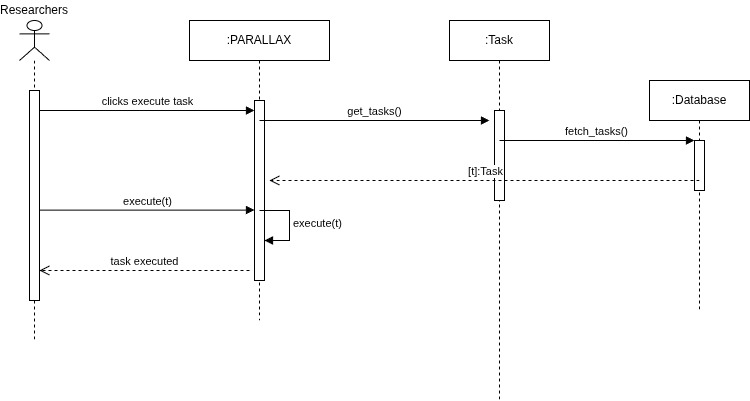
\includegraphics[width=1\textwidth]{images/parallax-ExecuteTask.jpg.jpeg}
    \caption{Diagramme de séquences technique — Exécution d'une tâche}
    \label{fig:seq_tech_execute}
\end{figure}

\begin{figure}[H]
    \centering
    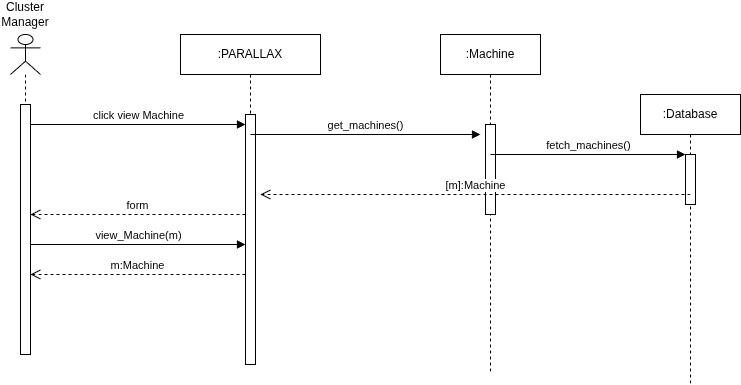
\includegraphics[width=1\textwidth]{images/parallax-consulter_machines (1).jpg.jpeg}
    \caption{Diagramme de séquences technique — Consultation des machines}
    \label{fig:seq_tech_machines}
\end{figure}

\begin{figure}[H]
    \centering
    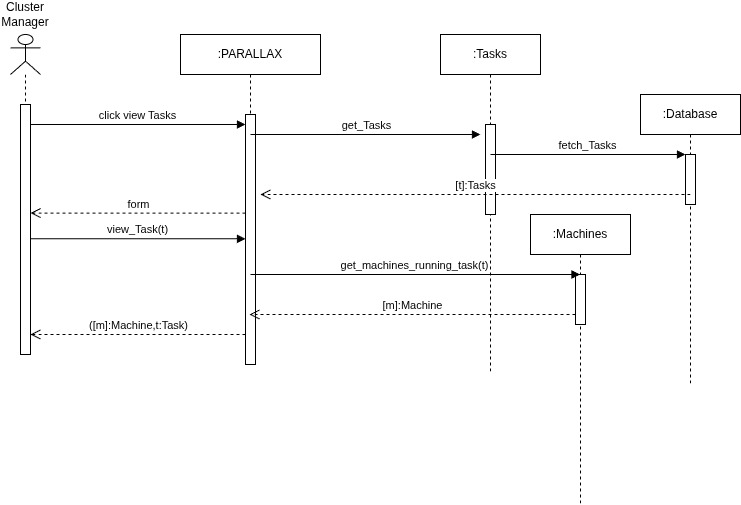
\includegraphics[width=1\textwidth]{images/parallax-consulter_taches (1).jpg.jpeg}
    \caption{Diagramme de séquences technique — Consultation des tâches}
    \label{fig:seq_tech_taches}
\end{figure}

\begin{figure}[H]
    \centering
    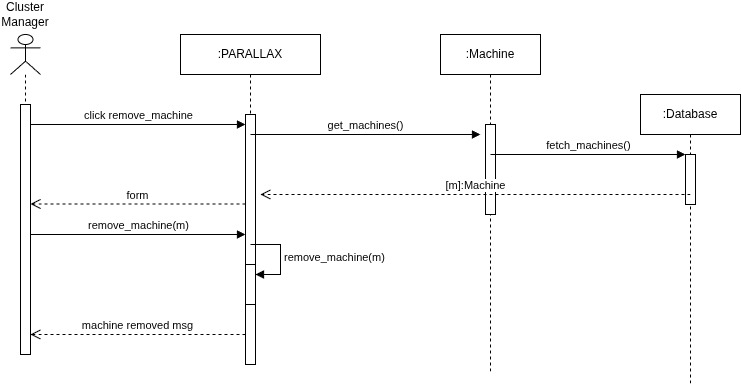
\includegraphics[width=1\textwidth]{images/parallax-Remove_Node.jpg.jpeg}
    \caption{Diagramme de séquences technique — Suppression d'un nœud}
    \label{fig:seq_tech_remove}
\end{figure}

\subsection{Protocoles de communication et coordination}

\subsubsection{Communication inter-agents}

Dans SMA\_PARALLAX, la communication entre agents est \textbf{directe et asynchrone}, reposant sur des messages structurés transportés via TCP sur le réseau local. Chaque message est un acte de communication au sens des ACL : il porte un performatif décrivant l'intention de l'émetteur, un émetteur, un récepteur, un contenu et un identifiant de conversation.

\begin{table}[H]
\centering
\renewcommand{\arraystretch}{1.3}
\begin{tabular}{|l|l|l|l|}
\hline
\textbf{Type} & \textbf{Performatif} & \textbf{Direction} & \textbf{Fonction} \\
\hline
Assertif & \textit{inform} & Worker $\rightarrow$ Contrôleur & Signalement d'état de charge via heartbeat \\
\hline
Directif & \textit{request} & Master $\rightarrow$ Worker & Demande d'exécution d'un sous-calcul \\
\hline
Notification & \textit{notify} & Contrôleur $\rightarrow$ Master & Alerte de défaillance détectée \\
\hline
\end{tabular}
\caption{Types de messages ACL dans SMA\_PARALLAX}
\label{tab:messages_acl}
\end{table}

\paragraph{Structure d'un message de heartbeat}

\[
\mathrm{HB}(i, t) = \big( \mathrm{uuid}_i,\; k_i(t),\; \widehat{\mathrm{CPU}}_i(t),\;
\widehat{\mathrm{RAM}}_i(t),\; q_i(t),\; \mathrm{Score}(i,t),\; \sigma_i,\; L_i(t) \big)
\]

Chaque nœud $n_i$ émet un heartbeat unicast vers le Contrôleur toutes les $T_{\mathrm{HB}} = 2$\,s. Il transporte la télémétrie nécessaire à l'orchestration : charge CPU et RAM, longueur de la file de tâches, score courant et état logique.

\paragraph{Architecture à deux couches}

\textbf{Couche 1 — heartbeat unicast vers le Contrôleur.} Signal périodique de présence et de télémétrie sur le canal best-effort.

\textbf{Couche 2 — gossip inter-pairs.} Toutes les $T_G = 5$\,s, chaque nœud envoie à $k = \lceil \log_2 N \rceil$ pairs aléatoires un résumé de sa vue récente du cluster.

\begin{figure}[H]
\centering
\begin{tikzpicture}[
    leader/.style={circle, draw=red!70!black, thick, minimum size=1.3cm,
                   fill=red!15, font=\bfseries},
    worker/.style={circle, draw=blue!70!black, thick, minimum size=1.1cm, fill=blue!10},
    hb/.style={->, thick, red!60!black},
    gossip/.style={dashed, thick, blue!50}
]
\node[leader] (L) at (0,0) {C};
\node[worker] (W1) at (90:3)   {$W_1$};
\node[worker] (W2) at (30:3)   {$W_2$};
\node[worker] (W3) at (-30:3)  {$W_3$};
\node[worker] (W4) at (-90:3)  {$W_4$};
\node[worker] (W5) at (-150:3) {$W_5$};
\node[worker] (W6) at (150:3)  {$W_6$};
\draw[hb] (W1) -- (L); \draw[hb] (W2) -- (L); \draw[hb] (W3) -- (L);
\draw[hb] (W4) -- (L); \draw[hb] (W5) -- (L); \draw[hb] (W6) -- (L);
\draw[gossip] (W1) to[bend left=15]  (W3);
\draw[gossip] (W2) to[bend right=20] (W5);
\draw[gossip] (W3) to[bend right=15] (W6);
\draw[gossip] (W4) to[bend left=20]  (W1);
\draw[gossip] (W5) to[bend left=15]  (W3);
\draw[gossip] (W6) to[bend right=20] (W4);
\begin{scope}[shift={(5.5,0)}]
    \node[font=\bfseries, anchor=west] at (0,1.5) {Légende};
    \draw[hb]     (0,1)   -- (1.2,1);   \node[anchor=west, font=\small] at (1.3,1)   {HB couche 1};
    \draw[gossip] (0,0.4) -- (1.2,0.4); \node[anchor=west, font=\small] at (1.3,0.4) {Gossip couche 2};
    \node[leader, minimum size=0.7cm, font=\small] at (0.2,-0.4) {C};
    \node[anchor=west, font=\small] at (1.3,-0.4) {Contrôleur};
    \node[worker, minimum size=0.7cm, font=\small] at (0.2,-1.2) {$W$};
    \node[anchor=west, font=\small] at (1.3,-1.2) {Worker};
\end{scope}
\end{tikzpicture}
\caption{Architecture à deux couches du heartbeat}
\label{fig:hb_2layers}
\end{figure}

\subsubsection{Coordination distribuée : élection du nœud remplaçant}

\paragraph{Objectif et déclencheurs}

Le protocole d'élection garantit la présence permanente d'un nœud \textbf{remplaçant} capable d'assurer la continuité en cas de défaillance d'un rôle critique. Trois événements déclenchent une élection :

\begin{itemize}
    \item[$\bullet$] \textbf{(D1) Démarrage à froid :} aucun remplaçant n'est présent dans le cluster.
    \item[$\bullet$] \textbf{(D2) Remplacement de rôle critique :} le Master ou le Contrôleur tombe en panne.
    \item[$\bullet$] \textbf{(D3) Stepdown du remplaçant :} maintenance, surcharge persistante ou réorganisation.
\end{itemize}

\paragraph{Fonction de score}

\[
score(n_i) =
a \cdot \frac{CPU_{libre} \cdot CPU_{total}}{CPU_{libre}^{max} \cdot CPU_{total}^{max}}
+ b \cdot \frac{RAM_{libre} \cdot RAM_{total}}{RAM_{libre}^{max} \cdot RAM_{total}^{max}}
+ c \cdot \frac{LATENCE_{min}}{LATENCE_i}
+ d \cdot \frac{freq_i}{freq_{max}}
\]

avec $a = 0{,}35$, $b = 0{,}35$, $c = 0{,}15$, $d = 0{,}15$.

\begin{algorithm}[H]
\caption{Initiation d'une élection par le nœud $k$}
\begin{algorithmic}[1]
\State $\sigma_k \gets electing$
\State $H \gets \{ j \in V \mid Score_{j,t} > Score_{k,t} \}$
\If{$H = \emptyset$}
    \State diffuser $coord(uuid_k)$
    \State $\sigma_k \gets leader$
\Else
    \ForAll{$j \in H$}
        \State envoyer $election(Score_{k,t}, uuid_k)$ à $j$
    \EndFor
    \State armer temporisation $T_{attente}$
\EndIf
\end{algorithmic}
\end{algorithm}

\begin{algorithm}[H]
\caption{Traitement des messages d'élection}
\begin{algorithmic}[1]
\Procedure{OnReceiveElection}{$s, u$}
    \If{$Score_{k,t} > s$ \textbf{ou} ($Score_{k,t} = s$ \textbf{et} $uuid_k > u$)}
        \State envoyer $alive$ à l'émetteur
        \State \Call{InitiateElection}{$k$}
    \EndIf
\EndProcedure
\Procedure{OnReceiveCoord}{$u$}
    \State $leader_k \gets u$
    \State $\sigma_k \gets normal$
\EndProcedure
\end{algorithmic}
\end{algorithm}

\subsubsection{Coordination distribuée : détection de panne}

\textbf{Phase 1 — Suspicion.} Si $\Delta_{ij}(t) \geq T_{\mathrm{suspect}}$, le nœud $i$ marque $j$ comme \textsc{suspected} et émet un \textsc{gossip\_query} à ses $k$ voisins.

\textbf{Phase 2 — Défaillance confirmée.} Si $\Delta_{ij}(t) \geq T_{\mathrm{failed}}$ et si la majorité des réponses sont négatives, $i$ marque $j$ comme \textsc{failed} et déclenche une élection si $j$ était le Master.

\begin{figure}[H]
\centering
\begin{tikzpicture}[
    ->, >=Latex, thick,
    node_state/.style={circle, draw=black!70, thick, minimum size=1.8cm, align=center}
]
\node[node_state, fill=green!15]  (A) at (0,0)  {\textsc{alive}};
\node[node_state, fill=yellow!25] (S) at (5,0)  {\textsc{suspected}};
\node[node_state, fill=red!15]    (F) at (10,0) {\textsc{failed}};
\draw (A) to[bend left=25]
    node[above, font=\small, align=center]
    {$\Delta_{ij} \geq T_{\mathrm{suspect}}$\\émettre \textsc{gossip\_query}} (S);
\draw (S) to[bend left=25]
    node[below, font=\small, align=center]
    {HB reçu\\\textbf{ou} gossip positif} (A);
\draw (S) to[bend left=25]
    node[above, font=\small, align=center]
    {$\Delta_{ij} \geq T_{\mathrm{failed}}$\\\textbf{et} $|R_{\mathrm{neg}}| \geq \lceil k/2 \rceil$} (F);
\draw (F) to[bend left=50]
    node[below, font=\small] {HB reçu (récupération)} (A);
\draw (A) to[loop above] node[above, font=\small] {HB reçu} (A);
\end{tikzpicture}
\caption{Machine à états — suivi d'un pair par un observateur}
\label{fig:fsm_panne}
\end{figure}

\subsubsection{Coopération dans l'exécution}

\paragraph{Inscription d'un nœud}

\begin{algorithm}[H]
\caption{Entrée d'un nœud dans le réseau}
\label{alg:node_join}
\begin{algorithmic}[1]
\State $N.ip \gets \textsc{DHCP\_REQUEST}()$
\State $N.uuid \gets \textsc{GENERATE\_UUID}()$
\State \textsc{STORE\_LOCAL}($N.uuid$)
\State \textsc{SEND\_BROADCAST}(\texttt{HELLO}, $N.uuid$, $N.ip$)
\If{le Contrôleur reçoit \texttt{HELLO}}
    \State \textsc{REGISTER\_NODE}($N.uuid$, $N.ip$)
    \State \textsc{SEND\_ACK}($N.uuid$)
\EndIf
\State \textsc{CONNECT}($N$, \textsc{CONTROLLER})
\end{algorithmic}
\end{algorithm}

\paragraph{Décomposition et distribution des calculs}

\begin{algorithm}[H]
\caption{Processus de décomposition}
\label{alg:decomposition}
\begin{algorithmic}[1]
\State Parser le programme et remplacer les annotations par les fonctions auxiliaires
\State Exécuter séquentiellement les sections non distribuées
\For{chaque section $S$ distribuée}
    \State Interroger le Contrôleur pour l'état des nœuds disponibles
    \State Calculer la répartition : $w_i = x_i / \sum_{j} x_j$
    \State Envoyer le programme instrumenté aux Workers sélectionnés
    \State Envoyer à chaque Worker le couple $(annotation\_id, data)$
\EndFor
\State Attendre tous les résultats (futex ou équivalent)
\end{algorithmic}
\end{algorithm}

\paragraph{Recomposition des résultats}

\begin{algorithm}[H]
\caption{Processus de recomposition}
\label{alg:recomposition}
\begin{algorithmic}[1]
\State Réceptionner les résultats partiels des Workers
\State Mettre à jour le compteur de complétion via futex
\If{tous les résultats attendus sont reçus}
    \State Appliquer la fonction \texttt{aggregate} définie par l'utilisateur
    \State Combiner les résultats partiels pour produire le résultat global
\Else
    \State Attendre les résultats manquants
\EndIf
\end{algorithmic}
\end{algorithm}

\begin{figure}[H]
    \centering
    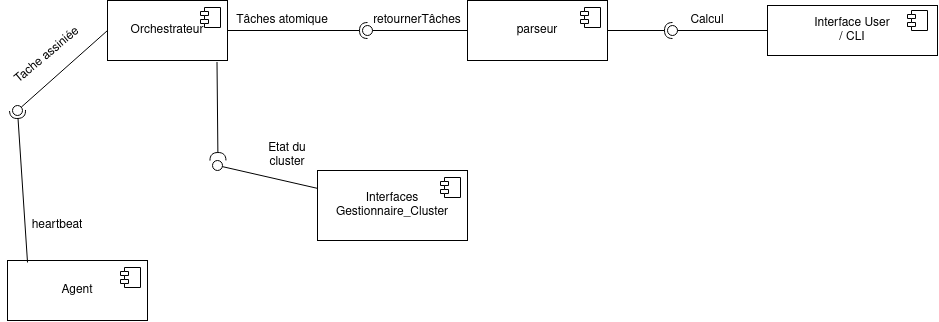
\includegraphics[width=1\textwidth]{images/Diagram des composants - parallax.drawio.png}
    \caption{Diagramme des composants}
    \label{fig:composants}
\end{figure}

% ==============================================================================
\chapter*{Conclusion Générale}
\addcontentsline{toc}{chapter}{Conclusion Générale}

Le projet PARALLAX, mené dans le contexte académique et scientifique de l'ENSPY, a permis de concevoir, modéliser et déployer avec succès une infrastructure de calcul distribué performante en exploitant un parc de machines locales hétérogènes et sous-exploitées.

L'adoption d'un formalisme centré sur les Systèmes Multi-Agents (SMA) s'est avérée déterminante pour surmonter les verrous technologiques liés à la dynamicité du cluster, à la détection proactive des surcharges et à la résilience automatique en cas de défaillance matérielle. En encapsulant les responsabilités de supervision, de décomposition et d'exécution au sein d'agents logiciels autonomes et communicants, PARALLAX offre une alternative locale privée, souveraine et économique aux infrastructures cloud externes.

Les résultats expérimentaux obtenus confirment non seulement une réduction drastique des temps de calcul pour les applications scientifiques lourdes, mais valident également les mécanismes de migration transparente des tâches en cas de panne critique. Les perspectives de ce travail résident dans l'intégration d'algorithmes d'ordonnancement prédictifs basés sur l'apprentissage par renforcement pour affiner au fil de l'eau l'allocation adaptative des charges au sein du réseau local de l'ENSPY.

\section*{Références}
\addcontentsline{toc}{chapter}{Références}

\begin{thebibliography}{99}

\bibitem{seti}
D. P. Anderson, ``SETI@home: An Experiment in Public-Resource Computing,''
\textit{Communications of the ACM}, vol. 45, no. 11, pp. 56--61, 2002.

\bibitem{htcondor}
D. Thain, T. Tannenbaum, and M. Livny,
``Distributed Computing in Practice: The Condor Experience,''
\textit{Concurrency and Computation: Practice and Experience}, vol. 17, no. 2--4, pp. 323--356, 2005.

\bibitem{tanenbaum_ds}
A. S. Tanenbaum and M. Van Steen,
\textit{Distributed Systems: Principles and Paradigms}, 2nd ed. Prentice Hall, 2007.

\bibitem{wooldridge}
M. Wooldridge,
\textit{An Introduction to MultiAgent Systems}. John Wiley \& Sons, 2009.

\bibitem{topcuoglu}
H. Topcuoglu, S. Hariri, and M.-Y. Wu,
``Performance-Effective and Low-Complexity Task Scheduling for Heterogeneous Computing,''
\textit{IEEE Trans. Parallel Distrib. Syst.}, vol. 13, no. 3, pp. 260--274, 2002.

\bibitem{kubernetes}
B. Burns, J. Beda, and K. Hightower,
\textit{Kubernetes: Up and Running}. O'Reilly Media, 2019.

\bibitem{bully}
H. Garcia-Molina,
``Elections in a Distributed Computing System,''
\textit{IEEE Trans. Computers}, vol. C-31, no. 1, pp. 48--59, 1982.

\end{thebibliography}

\section*{Annexes}

\end{document}